% !TEX TS-program = xelatex
% !BIB program = bibtex
% !TEX encoding = UTF-8 Unicode
% !Mode:: "TeX:UTF-8"
 \documentclass[bachelor, nocolorlinks, printoneside]{seuthesis} % 本科
% \documentclass[master]{seuthesis} % 硕士
% \documentclass[doctor]{seuthesis} % 博士
% \documentclass[engineering]{seuthesis} % 工程硕士
\usepackage{CJK,CJKnumb}
\usepackage{amsmath}
\usepackage{amsfonts} 
\usepackage{bm} 
\usepackage{algorithm}
\usepackage{algorithmicx}
\usepackage{algpseudocode}
\usepackage{stmaryrd}
\usepackage{placeins}
\usepackage{makecell}
\usepackage{graphicx,subcaption}
\usepackage{booktabs}
\newtheorem{theorem}{定义}
\usepackage{xcolor}
%\usepackage{algorithm,algpseudocode}

\newcommand\TODO[1]{\textcolor{blue}{#1}}

\floatname{algorithm}{算法}
\renewcommand{\algorithmicrequire}{\textbf{输入:}}
\renewcommand{\algorithmicensure}{\textbf{输出:}}
 % 这里是导言区

\begin{document}
\categorynumber{000} % 分类采用《中国图书资料分类法》
\UDC{000}            %《国际十进分类法UDC》的类号
\secretlevel{公开}    %学位论文密级分为"公开"、"内部"、"秘密"和"机密"四种
\studentid{04216747}   %学号要完整,前面的零不能省略。

\title{基于深度学习的三维重建和点云生成}{}{SEU Thesis \LaTeX Template}{subtitle}
\author{周烨凡}{Yefan Zhou}
\advisor{杨绿溪}{教授}{No Name}{Prof.}
\department{信息科学与工程学院}{Radio}
\major[12em]{信息工程}
\duration{2020年1月-2020年5月}

%\advisor{无名氏}{教授}{No Name}{Prof.}



\maketitle

\begin{abstract}{三维重建,点云,深度学习,数据挖掘}

    单视角三维物体形状重建(Single-view 3D Reconstruction)是三维视觉领域一直以来的核心问题之一。由于拟合非线性方程和学习模式的有效性,深度神经网络被期望在重建三维非线性形状的任务中表现出色。本课题探究了深度神经网络在三维重建任务中的有效性和内在机制,主要的工作和创新如下:
        
        \begin{enumerate}
            \item[1.] 针对基于自编码器结构的深度神经网络梯度过小等问题,提出采用多任务训练对编码器进行初始化,以及引入残差层这两种方法优化网络架构。在ShapeNet公开数据集上进行测试,取得了优于基于检索的非学习方法Oracle Nearest Neighbor的结果。
            \item[2.] 为了衡量三维数据集的聚类程度,提出了基于affinity propagation和silhouette score的度量标准,该方法得到的量化结果与数据集降维后的可视化结果吻合。
            \item[3.] 提出了影响三维重建任务中深度神经网络内在机制的主要因素是数据集的本质特征:当训练集中的三维形状集有相比于图片集更高的聚类程度的结构时,在这个数据集上训练的深度神经网络更有可能会执行识别机制而非重建机制,并定性和定量的证明了这一强相关性。
        \end{enumerate}
    最后,本文分析了上述结论对三维重建任务中的数据收集和神经网络训练的指导意义。
    \end{abstract}

\begin{englishabstract}{3D Reconstruction, Point Cloud, Deep Learning, Data mining}
    Single-view 3D reconstruction is one of the elementary tasks in the field of 3D vision. Due to the effectiveness in learning and approximating non-linear function, deep neural networks are expected to perform well on the task of reconstructing 3D nonlinear shapes. This paper investigates the effectiveness and internal mechanism of deep neural network in 3D reconstruction task. The main contribution and innovation are summarized as follows:
    \begin{enumerate}
        \item[1.] For the problem that the variance of multiple training results of deep neural network based on auto-encoder structure is too large, it proposes to leverage multi-task training to initiate the encoder and introduce residual layer to deepen the decoder in order to optimize network architecture. These methods are trained and tested on ShapeNet public dataset and they outperform the non-learning method based on retrieve, namely Oracle Nearest Neighbor. 
        \item[2.] Define novel way to measure clustering coefficient of 3D reconstruction dataset based on affinity propagation and silhouette score, the quantitative results of this metric is corresponding to qualitative results of visualization of dataset in low dimension.
        \item[3.] It claims that the bias of internal mechanism of network is mainly affected by the intrinsic properties of dataset: when the training set of 3D shapes has a more clustered structure than images, the deep neural networks trained on this dataset become more likely to perform recognition than reconstruction, and it proves the strong correlation between the deep neural networks and dataset property both qualitatively and quantitatively.
    \end{enumerate}
    Finally, this paper analyzes the significance of the above conclusions for data collection and neural network training.
\end{englishabstract}

\tableofcontents

% \begin{terminology}
% \begin{table}[h]
% \renewcommand\arraystretch{1.5}
% %\Large
% \begin{tabular}{>{\LARGE}m{0.2\textwidth} <{\centering}m{0.7\textwidth}}
% a & 如同汉字起源于象形,拉丁字母表中的每个字母一开始都是描摹某种动物或物体形状的图画\\

% b&和A一样,字母B也可以追溯到古代腓尼基。在腓尼基字母表中B叫beth,代表房屋,在希伯来语中B也叫beth,也含房屋之意。\\

% c& 字母C在腓尼基人的文字中叫gimel,代表骆驼。它在字母表中的排列顺序和希腊字母Γ(gamma)相同,实际上其字形是从后者演变而来的。C在罗马数字中表示100。\\

% d&D在古时是描摹拱门或门的形状而成的象形符号,在古代腓尼基语和希伯来语中叫做daleth,是“门”的意思,相当于希腊字母Δ(delta)。\\

% \end{tabular}
% %\caption{my table}
% \end{table}
% \end{terminology}


\begin{Main} % 开始正文

\chapter{绪论}
%\emph{在泛函分析中,卷积、旋积或摺积(英语:Convolution)是通过两个函数f 和g 生成第三个函数的一种数学算子,表征函数f 与g经过翻转和平移的重叠部分的面积。}

\section{课题的背景和意义}
基于单视角二维图片输入进行三维物体形状重建是三维视觉领域的核心问题之一,它能有效解决现实世界中二维数据丰富而三维数据稀少的问题,满足无人驾驶,智能建造,机器人领域的需求。点云数据具有易处理,易存储,易获得的特点,因此成为重建任务中常用的三维数据表示之一。

使用深度学习来进行单视角三维重建持续受到人们的关注。尽管很多的文章已经展示了创新的深度学习框架来提高三维重建任务中的最高水平\cite{li2018point,park2019deepsdf,fan2017point,tatarchenko2017octree,groueix2018papier,yang2018foldingnet,wang2018pixel2mesh,sun2018pix3d,tulsiani2017multi,wu2017marrnet,yan2016perspective},但很少有文章来尝试探究这些任务的本质特性。不可否认的是,重建三维非常规形状的问题已经变成了一个新的机器学习范例, 并且从事者使用的处理数据和训练网络的方法与在常规数据上的学习使用的方法不同(比如,Adam\cite{kingma2014adam}的使用频率比SGD要高)。因此,神经网络在三维重建学习这个新范例上怎样进行学习?是否与传统的向量分类和回归问题不同?

最近, \cite{tatarchenko2019single}的作者针对上述问题提出了一个让人惊讶的观点。他们尝试性的展示了当前最先进的用于三维重建任务的深度神经网络更倾向于通过首先分类输入图片到一个特定的簇,然后生成对应簇的平均三维形状,以此来进行预测。支持这一观点的主要实验证据是这些深度神经网络的三维预测结果与纯粹基于聚类和基于检索的基准模型的三维预测结果效果相近。这是一个非常有趣的观察,因为它说明了对于三维重建的任务来说,深度神经网络倾向于记住平均形状并且将其与图片输入的语义联系起来,而不是使用几何方法来生成一个形状,比如通过融合细粒度的局部结构形成一个整体形状。如果这个观点是正确的,这说明对于三维重建任务来说,最先进的深度神经网络实际执行了一个记忆任务而不是一个泛化任务\cite{arpit2017closer}。

本课题旨在优化三维重建任务中深度神经网络的架构,证实其有效性。同时进一步探究深度神经网络在三维重建任务中的内在机制,分析导致其偏倚于识别或重建机制的因素,这一研究将会帮助当前应用于三维重建的深度学习方法避免陷入识别机制的误区,同时也探讨了深度学习的本质问题,即如何帮助神经网络进行更好的泛化。

\section{研究现状}
\subsection{相关模型}
\cite{fan2017point}首次提出了以单张图片作为输入的三维点云重建任务中深度神经网络的基本架构, 即自编码器架构。编码器由卷积层和ReLU层构成,编码器的输入是一张图片和一个向量,向量用来模拟重建任务中的不确定性。解码器由全连接层构成,解码器输出点云的坐标,用 N × 3 的矩阵表示,N 为一个点云中三维点的数量。
\cite{yang2018foldingnet}提出了以三维点云作为输入的三维点云重建任务中深度自编码器的架构,创造性的提出用折叠的思想来生成点云,并重建三维形状,根据该思想实现的解码器仅使用了全连接层解码器的7\%的参数量,却在重建效果上超过当时的基准模型。
\cite{tatarchenko2019single}中评估了多个效果拔尖的单视角三维重建深度神经网路模型,并提出了基于识别和检索机制的多个非深度学习方法模型,且这些模型的重建性能超过了
当前的深度学习网络模型,这使得深度学习在单视角三维重建中的有效性受到了置疑。

\subsection{相关数据集}
ShapeNet\cite{chang2015shapenet}是一个注释丰富且规模较大的三维形状数据集,涵盖55个常见的类别,有大约5万个样本,每个样本内有一个三维模型和多张从不同视角渲染的该三维模型的图片,三维模型的数据格式为网格、体素,图片格式为PNG,在进行单视角三维重建时会从多个视角图片中选择一个视角的图片,因此这种情况下每个样本内有一张图片与一个三维模型。该数据集的创立者在ICCV 2017 举办了基于该数据集的单视角三维重建任务的竞赛,并将当时的基准成绩发表在\cite{Yi2017LargeScale3S}。
\cite{tatarchenko2019single}提供的数据集在ShapeNet\cite{chang2015shapenet}的基础上增加了点云数据格式,每个三维形状由9000多个点构成。共有52430个样本,涵盖55个类。
\subsection{神经网络学习机制}
深度神经网络是执行记忆还是泛化一直是现代机器学习中的主要问题。与我们将要介绍的类似,众所周知的猜测是优化过程是‘内容感知’的,并且取决于数据本身的属性\cite{arpit2017closer}。\cite{arpit2017closer}中还显示,训练期间的某些正则化技术可帮助深度神经网络泛化而不是记住任务。对于三维形状重建,\cite{tatarchenko2019single}表明神经网络倾向于记忆平均形状,而不是在几何意义上进行重建。确实,许多作品还显示了平均形状和识别信息在提高三维重建效果中的有效性\cite{kanazawa2018learning,pontes2018image2mesh,kurenkov2018deformnet}。

相比之下,也有很多作品利用三维形状的连续潜在空间中的分布信息\cite{li2018single,gwak2017weakly,sinha2017surfnet,li2018point,wu2018learning,yang20173d,yang2019pointflow}来提高三维重建效果,这超出了基于识别的范围。值得注意的是,\cite{wu2016learning,girdhar2016learning}表明形状算术可以在三维形状的潜在空间中进行,从而排除了神经网络仅在此问题设置中执行识别的可能性(因为执行算术需要的不是均值信息离散簇的形状)。其他一些工作建议通过将每个形状分解为部分\cite{tulsiani2017learning,niu2018im2struct,sung2017complementme}或通过连续过程\cite{sun2018pointgrow,choy20163d}来生成三维形状,这也超出了简单的识别任务。但是, \cite{wu2016learning,achlioptas2017learning,yang2018foldingnet}的作者将基于三维重建的自动编码视为点云上无监督分类的基础。尽管这些作品中的输入数据是三维形状,而不是二维图像,但是形状信息有助于分类的事实似乎确实增强了这样的概念,即三维重建更着重于识别而不是重建。尽管如此,形状信息有助于识别的事实不能成为判断三维重建网络所学知识的主要理由。有意义的未来方向是研究分别用于无监督分类和受监督三维形状重建的神经网络学习之间的差异,因为这两个方向的主要目标并不完全相同。

注意三维重建问题可以被看作是一个更普适的分布学习\cite{oliva2013distribution,poczos2013distribution}的特殊情况。但是,与分布学习中的理论工作如拓展核方法到回归分布不同,我们的工作集中于深度学习。即便如此,使人感兴趣的是能看到分布学习的传统工作把输出分布当做一个所有训练分布样本的连续线性组合直接处理,而不是使用两步法,预测簇索引后再预测平均分布。
\section{本文研究内容}
\subsection{课题关键问题以及难点}
首先,正式定义本课题的关键问题:一、优化深度神经网络框架,使其在单视角三维重建任务中超过基于识别机制的非深度学习方法,证明其有效性。二、讨论深度神经网络在单视角三维重建任务中执行的是识别机制还是重建机制。初步猜想是影响其在两者之间偏倚的因素为训练数据集的整体特征:聚类程度。因此本课题需要考虑以下几个难点:
\begin{enumerate}
    \item[1.]改进当前作为基准的神经网络架构以获得更好的重建性能。我们希望能对当前作为基准线的深度神经网络进行网络结构优化,以期望其在公认的标准数据集上能接近并超越基于识别机制的非深度学习方法。因此我们考虑借鉴图像领域成熟且有效的神经网络架构优化方法和训练技巧。
    \item[2.]定义神经网络的识别与重建这两种机制的数学表达,并用具体的实验结果来描述。
    \item[3.]设计并产生具有量化特征的三维重建数据集。为了探究神经网络训练集和网络的性能之间是否有强相关性,需要能定量的操控数据集的某些整体特征,如聚类系数。可以考虑的方式就是生成自定义的数据集,同时在生成过程中通过采样改变整体特征。为此可以考虑使用计算机图形学的相关软件来合成三维模型,并探究一些能进行不同三维形状之间插值的算法。
    \item[4.]定义衡量数据集指标的度量标准。在解决问题三后,需要构建一个度量标准来衡量数据集的聚类趋势,得到量化评分。   
\end{enumerate}
\subsection{主要贡献}
在这项工作中,我们定量和定性的展示了\cite{tatarchenko2019single}的结论不是通用的,而且这是一个不合适的数据集收集和不合理的数据使用导致的复杂结果。我们建议使用数据挖掘中确立已久的理论测量一个数据集的“聚类趋势”,称为affinity propagation~\cite{wang2008adaptive}和silhouette score~\cite{van2015using}, 并且我们展示了当用于训练三维重建任务的数据集不具有聚类特征时,训练结束的神经网络可以学会更集中在重建而不是识别。更重要的是,我们展示了即使是现实数据集如ShapeNet \cite{chang2015shapenet}, 在其上进行训练的神经网络依然呈现出重建机制,且通过优化网络架构和使用训练技巧,其重建效果接近并超过了基于检索的非深度学习方法。我们关于识别与重建这两种机制的理解更丰富,将三维重建的内在机制与数据以及训练过程相关联。之更具体的是,我们展示了训练集中的三维形状之间应该比训练集中的图片间呈现出更多的差异,以此来避免产生一个基于识别的机器学习模型。这一结论很实用,因为它为三维数据集的收集以及三维重建训练提供了指导。
\section{论文组织结构}
本论文主要有六个章节,各章的内容安排如下:
\begin{itemize}[\hspace{2cm}]
    \item[第一章] 绪论,简要介绍了单视角三维重建任务的研究背景和意义,并对现行的相关理论,模型和数据集进行简单概述与分析。介绍本论文的研究思路、关键问题以及主要贡献。
    \item[第二章] 问题与定义,介绍了本论文探究的损失函数和算法的理论基础。给出了重建机制与识别机制的数学定义。
    \item[第三章] 模型,详细介绍了基准模型,以及优化模型的架构,并给出了网络在ShapeNet大型数据集上训练的过程信息以及训练结果的分析比较。
    \item[第四章] 机制分析,给出了机制探究的理论基础与实验设计,介绍了自定义数据集的制作,网络在自定义数据集上训练的过程信息以及训练结果的定性与定量分析。
    \item[第五章] 总结与展望,分析并总结本课题研究成果的总体优缺点,并提出未来的研究改进方向。
\end{itemize}
\chapter{问题与定义}
\section{问题描述}
我们探究的问题是从单张图片重建一个三维形状。输入$I$是一张二维RGB图片。输出$S$由一个点云表示。我们在本课题中不考虑基于体素的体积表达。对于基于点云的表达,
每个形状$S$是一个包含三维点的点集。一个神经网络在训练中通过减小特定损失函数定义的经验损失$l$,以此来从输入图片$l$预测形状$S$。
\begin{equation}
    \min_f \sum_{i=0}^{n-1} {l(f(I_i), S_i)}.
\end{equation}
我们想通过优化$f$,使其在训练数据集上训练后,在测试数据集上取得更低的平均损失。同时,我们还想学习$f$的特性来了解它执行的是一个重建任务还是识别任务。
两个指标被用来测量重建结果$\widehat{S} = f(I)$与标签点云$S$之间的差异,称为Chamfer Distance和F-score。

\noindent
\textbf{Chamfer distance.}Chamfer Distane通过搜索另一个点集中最近点来测试一个点集到另一个点集的整体距离。
\begin{equation}\label{eqn:chamfer}
	d_{CH}(S,\widehat{S}) = \frac{1}{|S|}\sum\limits_{\mathbf{x}\in S}\min_{\widehat{\mathbf{x}}\in \widehat{S}}\|\mathbf{x}-\widehat{\mathbf{x}}\|_2 + 
    \frac{1}{|\widehat{S}|}\sum\limits_{\widehat{\mathbf{x}}\in \widehat{S}}\min_{\mathbf{x}\in S}\|\widehat{\mathbf{x}} - \mathbf{x}\|_2.
\end{equation}
尽管Chamfer Distance是运算高效且方便的,它会被很小一部分异常点的强烈影响。所以我们也要如[26]建议的那样采用F-score来预测点集。

\noindent
\textbf{F-score.}另外一个衡量形状重建的指标是F-score, 该指标是精确度和回忆度的调和平均数。在给定相应的标签$S$,且在固定的距离阈值$d$内,重建点云$\widehat{S}$
的精确度$\textit{Prec}$为定义为:

\begin{equation} \label{eq:precision}
\textit{Prec}(\textit{d}, S, \widehat{S}) = \frac{1}{|\widehat{S}|} \sum_{r \in \widehat{S}} \llbracket \min_{s \in S} ||r-s || < \textit{d} \rrbracket,
\end{equation}
where $\llbracket \cdot \rrbracket$ is the Iverson bracket.
    
相似的,标签点云$S$对重建点云$\widehat{S}$的回忆度$\textit{Rec}$是:
\begin{equation} \label{eq:recall}
    \textit{Rec}(\textit{d}, S, \widehat{S}) = \frac{1}{|S|} \sum_{s \in S} \llbracket \min_{r \in \widehat{S}} ||s-r || < \textit{d} \rrbracket.
    \end{equation}

使用这两个量,如下计算F-score:
\begin{equation} \label{eq:f-score}
    \textit{F}(\textit{d}, S, \widehat{S}) = \frac{2 \times \textit{Prec}(\textit{d}, S, \widehat{S})\times \textit{Rec}(\textit{d}, S, \widehat{S})}{\textit{Prec}(\textit{d}, S, \widehat{S}) + \textit{Rec}(\textit{d}, S, \widehat{S})}.
\end{equation}
重建的准确度被精确度量化,用以测量重建的点集离标签点集有多近。重建的完整度被回忆度量化,用来测量标签点云多少部分被重建点云覆盖。
所以,一个高的F-score显示了重建是准确且完整的[12]。
\section{识别或重建}
在这个部分,我们正式定义本文中研究的两种学习范式,被称为识别(\emph{recognition})和重建(\emph{reconstruction})

\begin{theorem}\label{def:recognition}(识别)
    一个基于识别的神经网络$f$用两步预测形状重建。神经网络重建方程可以写成:
\begin{equation}
        \widehat{S} = f(I) = f_1(f_2(I)),
\end{equation}
方程中的$f_2(\cdot)$将输入图片映射到一个标量索引,并且$f_1(f_2(I))$将这个标量索引映射到索引$f_2(I)$对应的特定簇的平均形状。
\end{theorem}

\begin{theorem}\label{def:reconstruction}(重建)
    一个基于重建的神经网络直接进行三维重建。即\begin{equation}
        \widehat{S} = f(I),
    \end{equation}
并且重建不会明显的使用图片簇的任何信息。
因为当前最流行的单视角三维重建经常使用一个编码器-解码器结构,所以一个相似的概念是由编码器获得的码字不会形成簇。
\end{theorem}
\textbf{主要问题}

在这篇论文中,我们研究神经网络执行识别机制还是重建机制。我们展示了向两者任一偏倚的趋势由数据集特性决定。

注意\cite{tatarchenko2019single}的主要结论是单视角三维重建中的深度神经网络主要执行识别工作。换句话说,神经网络的方程更接近于定义\ref{def:recognition}而不是
定义\ref{def:reconstruction}。
\section{数据集的聚类趋势}
\label{sec:metric_on_dataset}
在这个部分,我们定义用来测量数据集聚类趋势的指标。具体来说,我们使用silhouette score~\cite{van2015using}来测量聚类趋势。
给定一个数据集$D = \{x_i\}_{i=0}^{N-1}$并且一个随机距离$d(x,y)$方程。我们考虑满足下面三个属性的任何距离方程,
$d(x_1,x_2)=d(x_2,x_1)$, $d(x_1,x_2)\ge 0$, 和 $d(x,x)=0$。在我们的实验中,我们使用Chamfer Distance作为点云的距离指标。
我们使用$\ell$-1距离作为图片之间的距离。我们能通过明确一个聚类特性方程$C(\cdot)$来确定一个数据集的\emph{聚类程度}。对于每个样本$x_i$,
聚类方程会给出一个聚类标签$C(x_i)$。我们使用$C(x_i)$来指示包含有$x_i$的簇,比如说,聚类标签$C_i$等价于$C(x_i)$。有时候,数据集
已经包含了标签聚类。更多情况下,聚类划分需要通过一个算法来获得。然后,第$i$个样本的轮廓系数(silhouette score)被定义为:
\begin{equation}
    s(i) = \frac{b(i)-a(i)}{\max(a(i),b(i))},
\end{equation}
其中
\begin{equation}
    a(i) = \frac{1}{|C_i|-1}\sum_{j\in C_i, j\neq i}d(i,j),\;\;\;\;\;
    b(i) = \min_{k\neq i}\frac{1}{|C_k|}\sum_{j\in C_k}d(i,j).
\end{equation}
聚类趋势, 以轮廓系数定义, 由以下方程得出:
\begin{equation}
    \textit{Clustering-tendency} = \frac{1}{N}\sum_i s(i).
\end{equation}

对于没有标签聚类的数据集,我们需要找到聚类方程$C(\cdot)$。在这篇论文中,我们使用affinity propagation~\cite{wang2008adaptive}
来进行聚类。Affinity propagation非常适合我们的设定,因为它不需要预先确定簇的数量,并且它使用一个预设的距离矩阵来
分配数据点$x_i$到一个簇$C_i$。我们使用~\eqref{eqn:chamfer}中的Chamfer Distance作为距离方程$d(x,y)$来处理
数据集中的无序点云。

\chapter{模型方法}
在这个部分,我们介绍了本文研究的三维重建任务中深度神经网络基准模型和非深度学习基准模型,并结合在ShapeNet上的实验结果对其优缺点进行分析。
基于这些分析,对深度神经网络基准模型进行优化,使其超过基于检索机制的非深度学习基准模型,证实了深度
学习的优越性,我们使用了这两种方法:
\begin{itemize}[\hspace{1cm}]
    \item[1.] 基于多任务训练的编码器初始化
    \item[2.] 引入残差层增加解码器深度
\end{itemize}
我们还展示了在真实数据集ShapeNet上,即使是一个标准的三维重建深度神经网络也倾向于执行重建任务而不是识别任务。我们
的结论基于两点观察:
\begin{itemize}[\hspace{1cm}]
    \item[1.] 首先,由标准的三维重建网络获得的量化结果如Chamfer Distance 和 F-score与基于Oracle-Nearest-Neighbor(Oracle-NN)
    的重建方法所获得的结果相近。
    \item[2.] 其次,由自编码训练获得的高维码字的2D T-SNE 可视化,和使用标签信息进行训练相比,并没有展示出明显的形成簇的趋势。
    而且,没有标签的重建效果比有标签的重建效果要更好。
\end{itemize}

在这个章节,我们使用的数据集均为ShapeNet, 共计55个类,52430个样本,训练集/验证集/测试集按照70\%/10\%/20\%随机采样划分。图片大小为$224 \times 224 $,
每个三维点云有1024个三维点构成。


\section{基准模型}
\subsection{模型介绍}
\subsubsection{非深度学习方法}

论文~\cite{tatarchenko2019single}中提出了以下三个基于识别机制的非深度学习模型:
\begin{itemize}
    \item \textit{Clustering}:通过对样本点云集使用聚类算法,将一组点云集划分为多个集群,每个集群内部计算一个平均
    三维形状,接着训练一个基于输入图片预测特定集群的分类器,将集群的平均三维形状作为预测结果。
    \item \textit{Retrieval}:借鉴了现有的基于图片检索对应物体的三维形状的方法~\cite{10.1145/2816795.2818071},在测试
    时,根据输入图片检索训练集中对应的三维点云,直接提取出来作为预测结果。
    \item \textit{Oracle-Nearest-Neighbor\footnote[1]{下文缩写为Oracle-NN}}:该模型在预测时,在训练集中直接搜索与标签点云损失最小的训练点云,将其
    作为预测结果。因为该模型在搜索最近点云时需要标签点云,而实际测试时只有对应的二维图片作为输入,所以在实践中是不可能
    实现的。
\end{itemize}

因为论文\cite{tatarchenko2019single}的实验结果表明Oracle NN的水平超过了所有当前最先进的
深度学习模型,而且它是表征任何实际基于检索的非深度学习方法的性能极限的理论基准。所以我们将其当做本课题的非深度学习基准模型, 并进行这样的实现\ref{alg:orcalenn}。
我们发现在将该模型应用到ShapeNet时,因为测试集有10000个样本,训练集有35000个样本,如果这样计算,复杂度很高,需要在GPU上消耗大概一周时间,占用了大量的计算资源。
于是考虑利用数据集自带的类标签,共计55个类,如车,床,椅子等,在每个类内数据集中运行该算法\ref{alg:orcalenn},大约10小时完成。

\begin{algorithm}
    \caption{Oracle Nearest Neighbor}
    \label{alg:orcalenn}
    \begin{algorithmic}[1] %每行显示行号
        \Require ${T^{n}_{i=0}}$测试集,${D^{t}_{j=0}}$训练集
        \Ensure ${R^{n}_{k=0}}$预测结果
        \State $i \gets 0$
        \State $k \gets 0$
        \While{$i<n$}
            \State $index \gets 0$
            \State $mindis \gets inf$
            \State $j \gets 0$
            \While{$j<t$}
                \State $dis \gets Distance(T_i, D_j)$
                    \If{$dis < mindis$}
                        \State $index \gets j$
                        \State $mindis \gets dis$
                    \EndIf
                \State $j \gets j+1$
            \EndWhile
        \State $R_{k=i} \gets D_{j=index}$
        \State $i \gets i+1$
        \EndWhile
    \end{algorithmic}
\end{algorithm}

\subsubsection{深度学习方法}
\TODO{先画流程图,可以的话画一下比较炫酷的图}
\begin{figure}
    \centering
    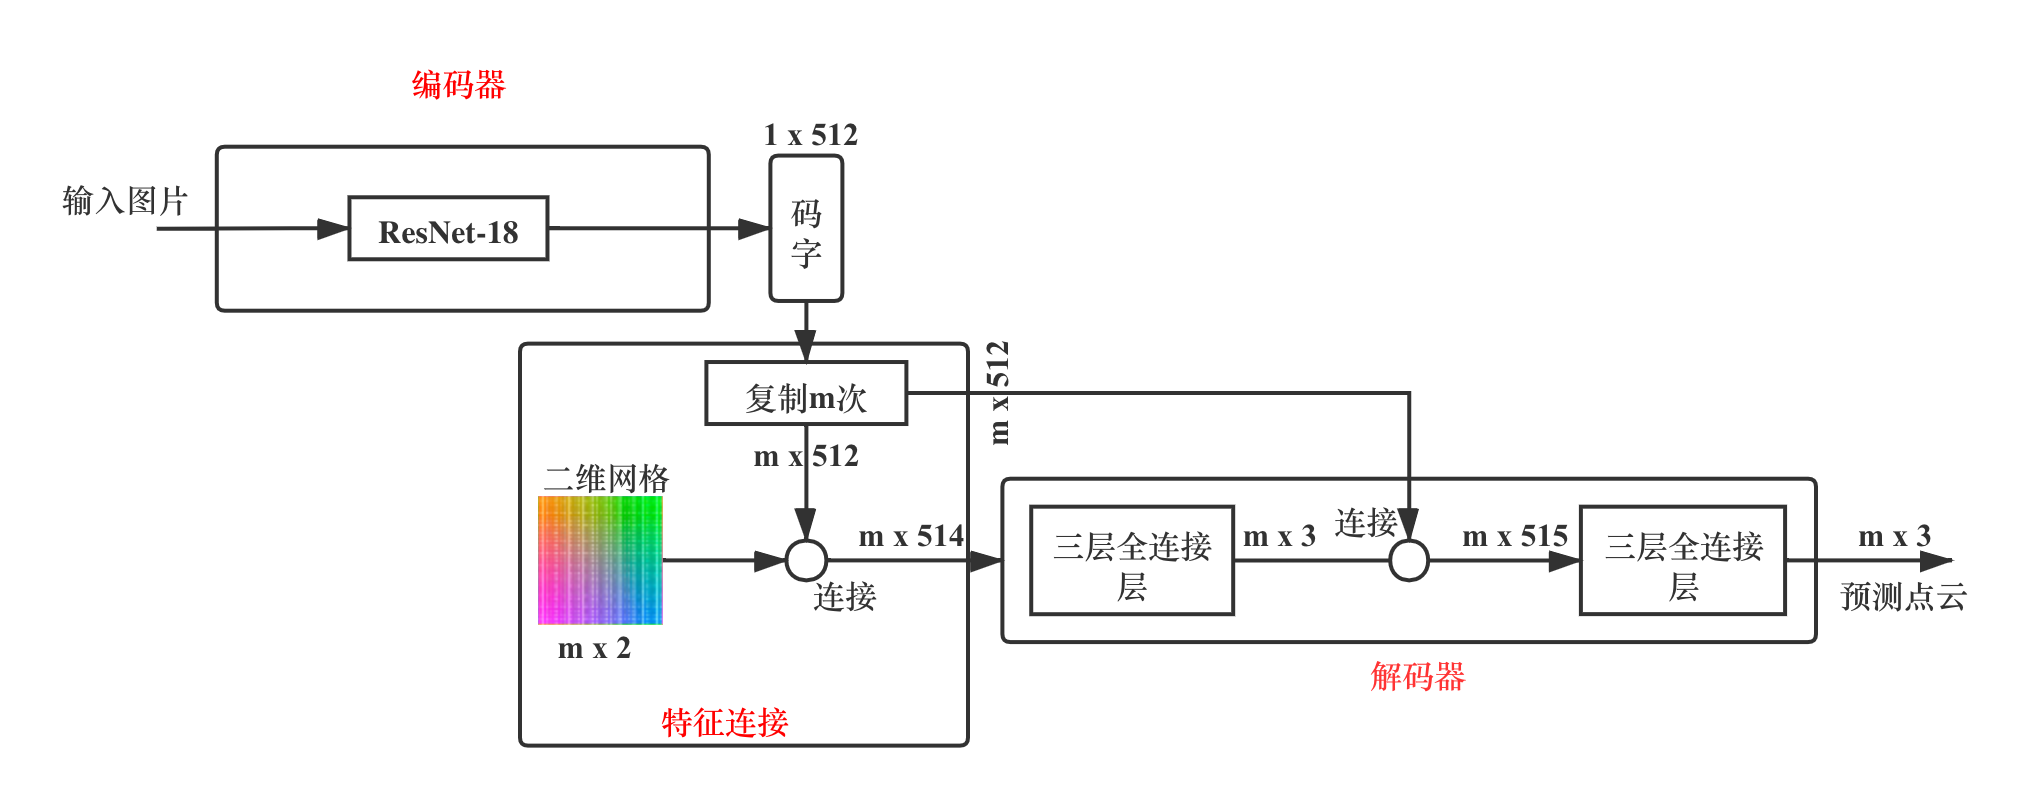
\includegraphics[width=0.99\textwidth]{figs/model/ae_baseline_grid.png} 
    \caption{基于自编码器架构的深度神经网络基准模型}
    \label{fig:ae_baseline}
\end{figure}
根据论文PSGN~\cite{fan2017point}提出的基于“编码器-解码器”架构\footnote[1]{下文简称为“自编码器”或“auto-encoder”}的深度神经网络模型,我们进行了如图\ref{fig:ae_baseline}的实现。网络的主要架构如下:
\begin{itemize}
\item 编码器:采用ResNet-18~\cite{He_2016}的卷积层架构作为接受二维图像输入并提取图像特征的编码器, 具体来说,移除ResNet-18最后一层用来分类的全连接层,将一维特征层直接输出作为码字。
\item 特征连接:模型中存储有一个预先初始化好的二维正方形网格点云,长宽在[-1,1]之间,由$m \times 2$的矩阵表示。在将码字输入解码器之前,
我们先将其复制$m$次,然后将$m \times 512$矩阵(码字)与$m \times 2$矩阵(二维网格)连接起来,连接的结果是大小为$m \times 514$的矩阵。
\item 解码器:采用FoldingNet解码器\cite{yang2018foldingnet}作为从码字恢复到点云结构的解码器,具体来说,这个解码器由两个感知器构成,每个感知器由三层全连接层构成。
\end{itemize}

该基准模型的关键部分是提出的解码器使用两个连续的3层感知器将固定的2D网格扭曲为输入点云的形状。这个过程称为折叠操作,实质上形成了通用的二维到三维映射。
为了直观地解释为什么这种折叠操作是通用的二维到三维的映射,请用矩阵$U$表示输入的二维网格点。$U$的每一行都是一个
二维网格点。用$U_i$表示$U$的第$i$行,用$\theta$表示编码器输出的码字。然后,在特征连接之后,解码器的输入矩阵的
第$i$行为$[u_i,\theta]$,由于感知器并行应用于输入矩阵的每一行,因此输出矩阵的第$i$行可以写成$f([u_i,\theta])$,其中
$f$表示感知器进行的功能。可以将该函数视为带有码字$\theta$的参数化高维函数,码字$\theta$是指导功能结构(折叠操作)的参数。由于多层感知器
擅长拟合非线性函数,因此它们可以在二维网格上执行精细的折叠操作。

\subsection{实验结果与分析}

我们展示了上述的深度学习基准模型和非深度学习基准模型在ShapeNet上的实验效果,并对此进行分析。
对于非深度学习基准模型Oracle-NN, 我们展示了所有重建样本的损失平均值作为量化的评估结果。
对于基于自编码器架构的深度学习基准模型,我们以Chamfer Distance\footnote[2]{Chamfer Distance数值越小说明重建效果越好}作为损失函数,使用Adam优化器,训练了100个周期,使其达到收敛,并对超参数进行调参,总共进行了8次训练,最终展示了
由所有重建样本的损失平均值表示的最优重建效果。两个模型的最优结果展示在表\ref{table:metric_per_baseline}。从这个结果中我们可以看出,在最优平均损失方面,Oracle NN
超过了深度神经网络,这一结果与论文\cite{tatarchenko2019single}中展示的两者之间的差距相吻合,而且正如前文所展示的,Oracle-NN是一个理论上的基于识别机制的基准模型,
无法应用于实际任务,所以这一优越结果是被预计的。但是,在训练的过程中,我们发现了神经网络基准模型的一些问题,这意味着有可能通过一些优化或者训练技巧来继续缩小这一差距。
结合图\ref{fig:lossplot}展示的在不同学习率下的两次训练过程的损失变化, 对主要问题的分析如下:
\begin{itemize}
    \item 神经网络训练状态不稳定。首先可以看出,学习率仅发生了三倍的变化,
        就使得网络陷入了与最优效果相差较大的局部最优,且Adam优化器也没有能使得网络跳出这个点。在正常情况下,网络不应该对超参数有如此高的敏感程度。同时,这也说明重建任务也许对
        参数初始化有比较高的要求。
    \item 神经网络架构的学习能力较弱。如图\ref{fig:testloss}所示,两个网络分别在第30周期和第60周期收敛,收敛过早说明当前的网络可能出现了训练过程中梯度过小的问题。
    \item 神经网络的编码器缺少显性的梯度优化。从理论角度来说,网络损失函数仅描述两个三维点云的相似程度,因此有理由怀疑该函数传播的梯度并不能给予对二维图片进行处理的
    编码器足够的优化指导,使其提取需要的图片特征。从实验角度来说,我们将编码器输出的码字进行了T-SNE降维可视化,如图\ref{fig:T-SNE2},可以看出
    编码器提取的特征码字并不具有区分图像类别的特征,虽然这不能证明编码器完全没有提取有助于三维重建的图像信息。
\end{itemize}

基于上述对神经网络基准模型的问题分析,我们将在下文对网络初始化以及梯度过小等问题提出优化方案。
\begin{table}
    \centering
    \caption{基准模型的评估结果}
    \label{table:metric_per_baseline}
    \begin{tabular}{cc} 
    \hline
    模型         & Chamfer Distance        \\ 
    \hline
    Oracle NN  & 0.0719                  \\
    自编码器(基准模型) & 0.0806 \\
    \hline
    \end{tabular}
\end{table}

\begin{figure}[!htb]
       \begin{subfigure}[t]{0.49\linewidth} \centering 
         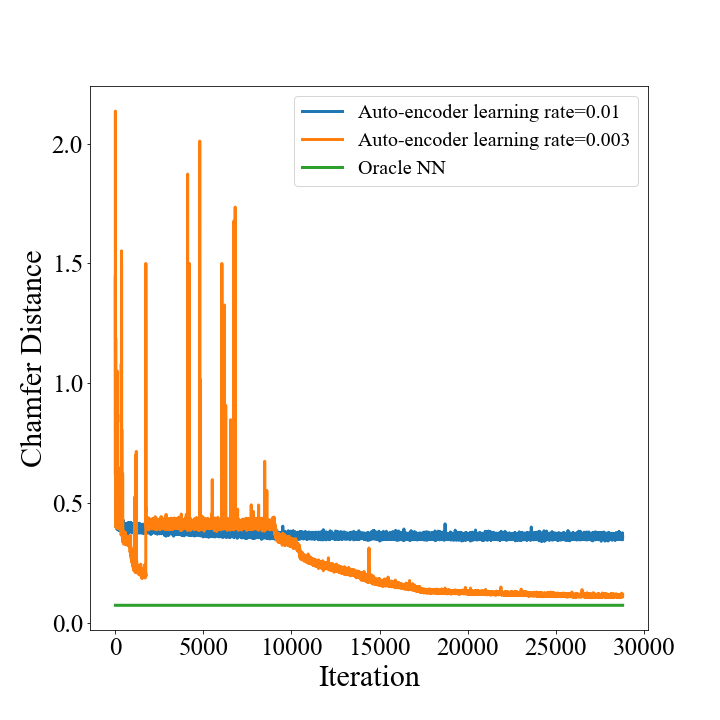
\includegraphics[width=\columnwidth]{figs/model/ae_trainingloss.png}
         \caption{训练集损失}\label{fig:trainingloss}
       \end{subfigure}
      \begin{subfigure}[t]{0.49\linewidth} \centering
          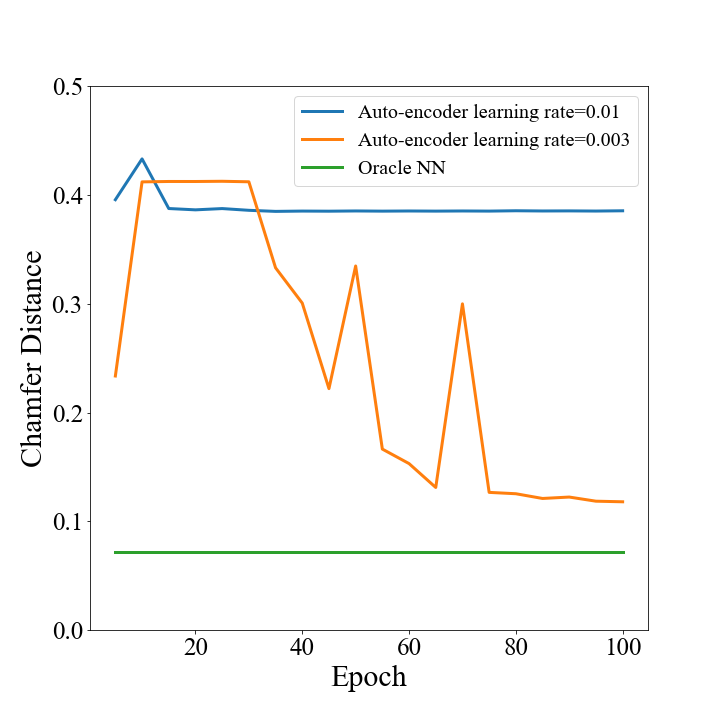
\includegraphics[width=\columnwidth]{figs//model/ae_testloss.png}
          \caption{测试集损失}\label{fig:testloss}
      \end{subfigure}
       \caption{\small 深度神经网络基准模型的两次训练过程。蓝色与橙色指同一网络在不同优化器学习率下的训练,绿色指非深度学习基准模型的量化结果}
    \label{fig:lossplot}
\end{figure}

\FloatBarrier
\section{模型优化}
\subsection{架构优化}
在这个部分,我们提出加入弱标签信息进行多任务训练,以及引入残差层这两种方法优化神经网络架构。
\begin{itemize}
    \item 针对如何给网络提供更优初始化,以及给予编码器显性优化的问题,我们提出加入弱标签信息来进行初始化的方法。在训练的前5个时期,在预测重建点云的同时将码字从中间层
抽出进行一次图像分类训练,在第6个时期以及之后取消这一操作。这一技巧能帮助编码器获得一个较好的初始化,
使得各个类别的码字具有类别独特性,帮助译码器进行类内重建,而类内的三维形状之间有很高的相似度,所以能较快的提高整体准确率。

    \item 针对深度神经网络梯度过小和消失的问题,我们在基准模型\ref{fig:ae_baseline}的译码器中引入残差层,将每个三层全连接层感知器改为
    由三个残差块组成的感知器,如图\ref{fig:resnet_decoder}残差块内部每个激活函数之前进行批处理归一化,译码器部分的参数量是之前的两倍,保留译码器之前编码器和特征连接结构不变。
    根据图像分类领域深度学习的经验,残差层和批处理归一化都能有效的解决反向传播中梯度过小和消失的问题,且可以在此基础上增加网络深度,提高重建能力。

\begin{figure}
    \centering
    \begin{tabular}{c@{}}
    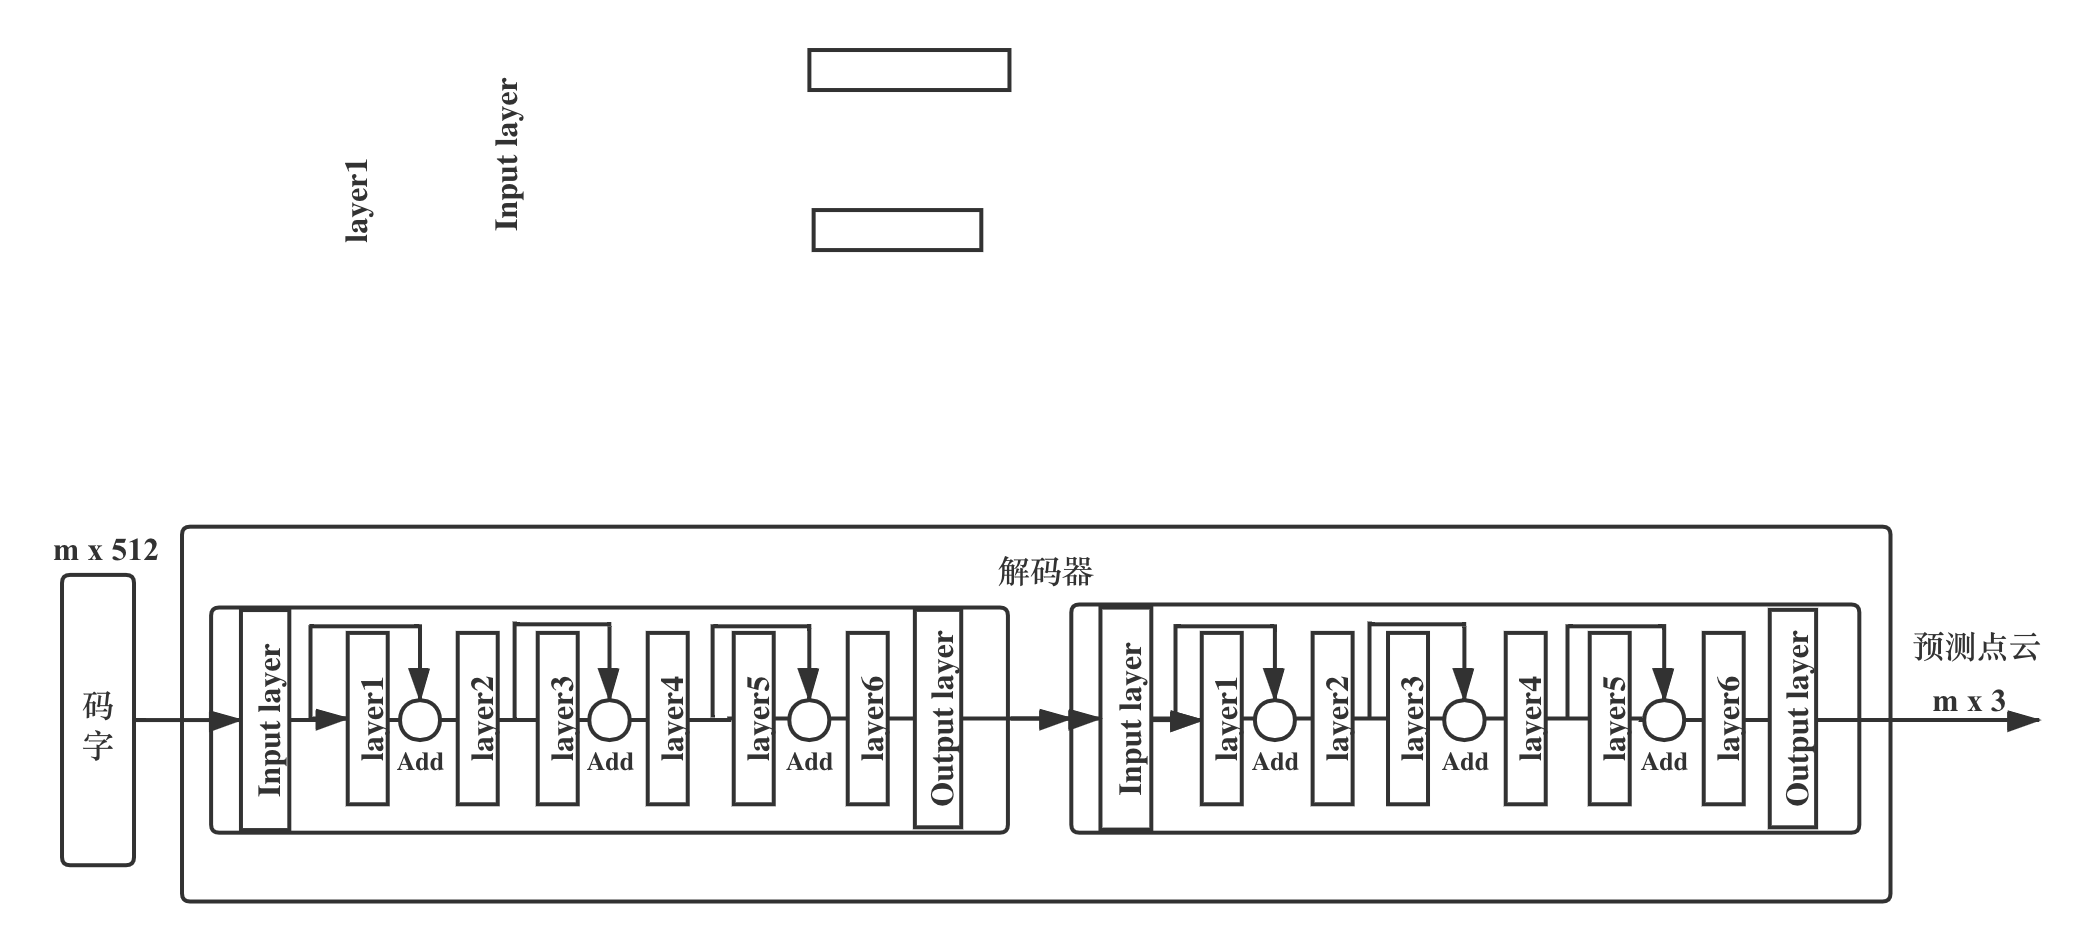
\includegraphics[width=0.99\columnwidth]{figs/model/resnet_decoder.png}
    \end{tabular}
    \caption{Evaluation metrics of reconstruction.  chamfer distance and earth mover's distance per shape. Auto-encoder based methods perform consistently across different classes. }
    \label{fig:resnet_decoder}
\end{figure}

\end{itemize}
\subsection{实验结果与分析}

\begin{table}
    \centering
    \caption{优化模型的评估结果}
    \begin{tabular}{ccc} 
    \hline
    模型                      & Chamfer Distance \\
    \hline
    自编码器(基准模型)            & 0.0806     \\
    自编码器(弱标签信息)           & 0.0716                             \\
    自编码器(残差层解码器)         & 0.0768                         \\
    Oracle NN & 0.0719                           \\
    \hline
    \end{tabular}
\end{table}


\subsubsection{重建效果}
\begin{figure}[!htb]
    \centering
    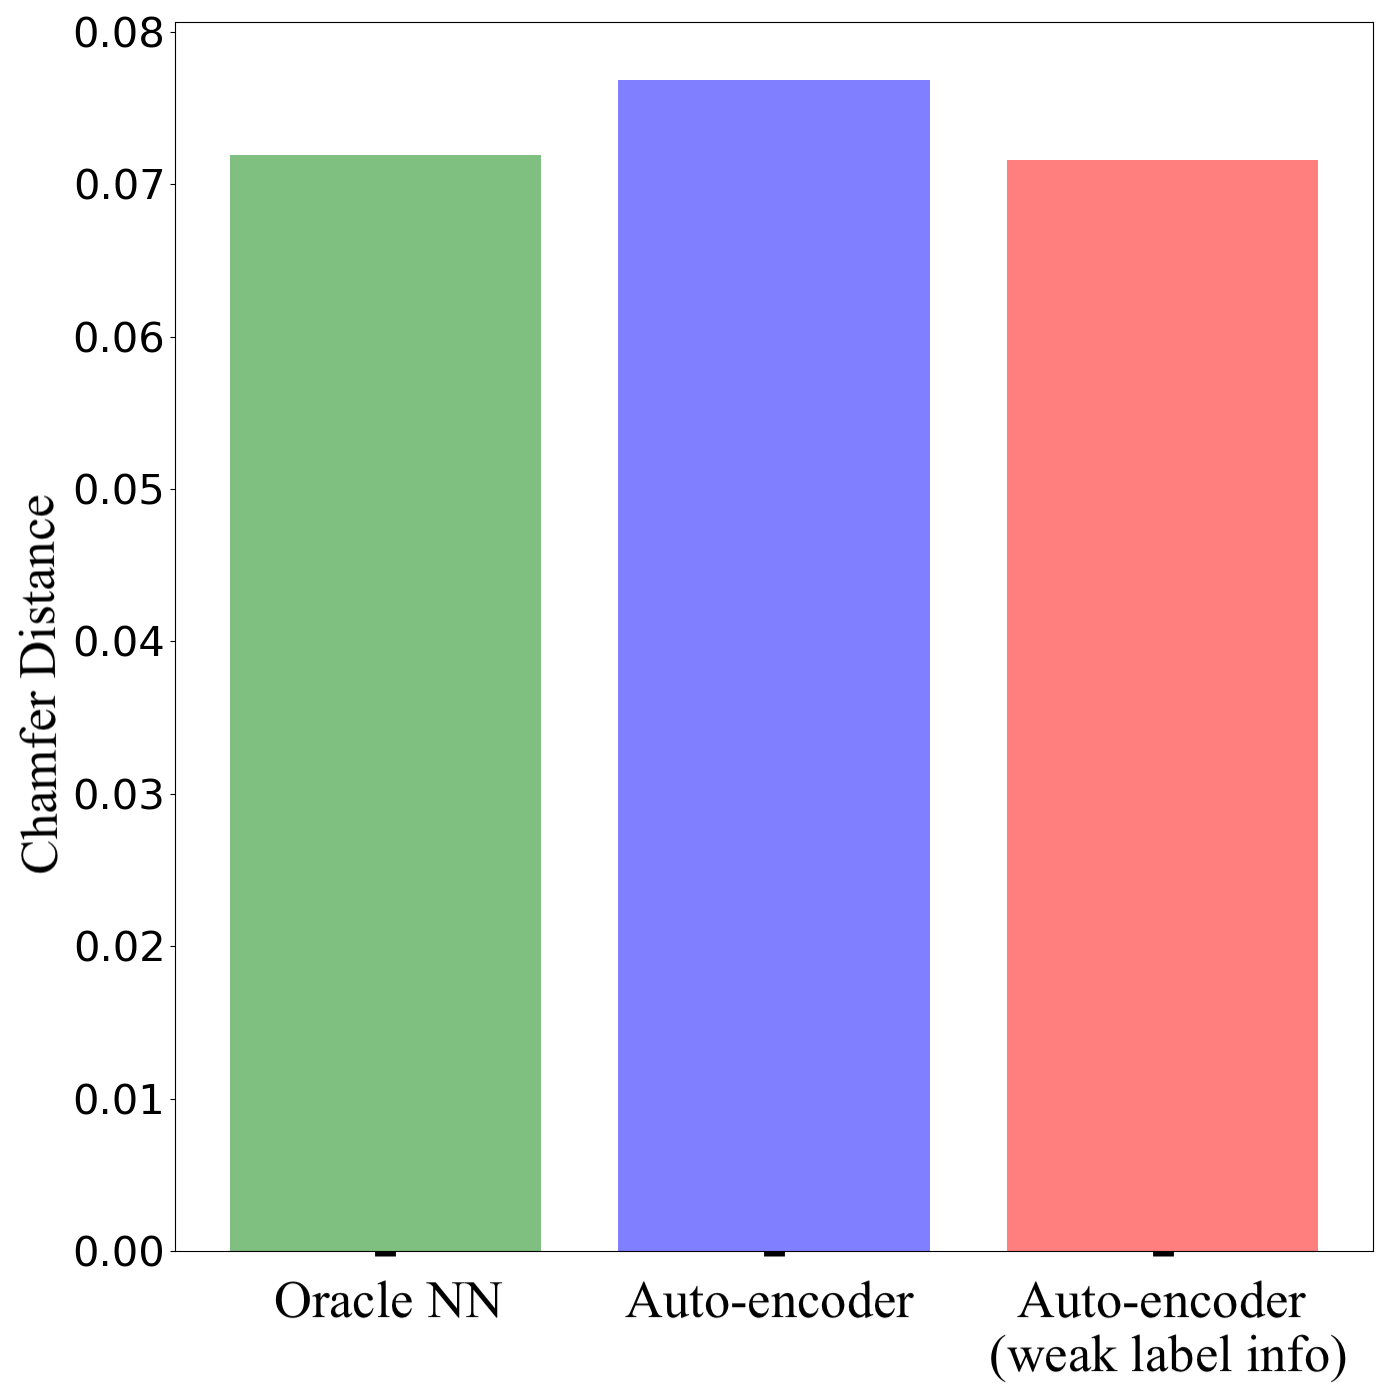
\includegraphics[width=.40\textwidth]{figs/chamfer-compare_roman.png}
    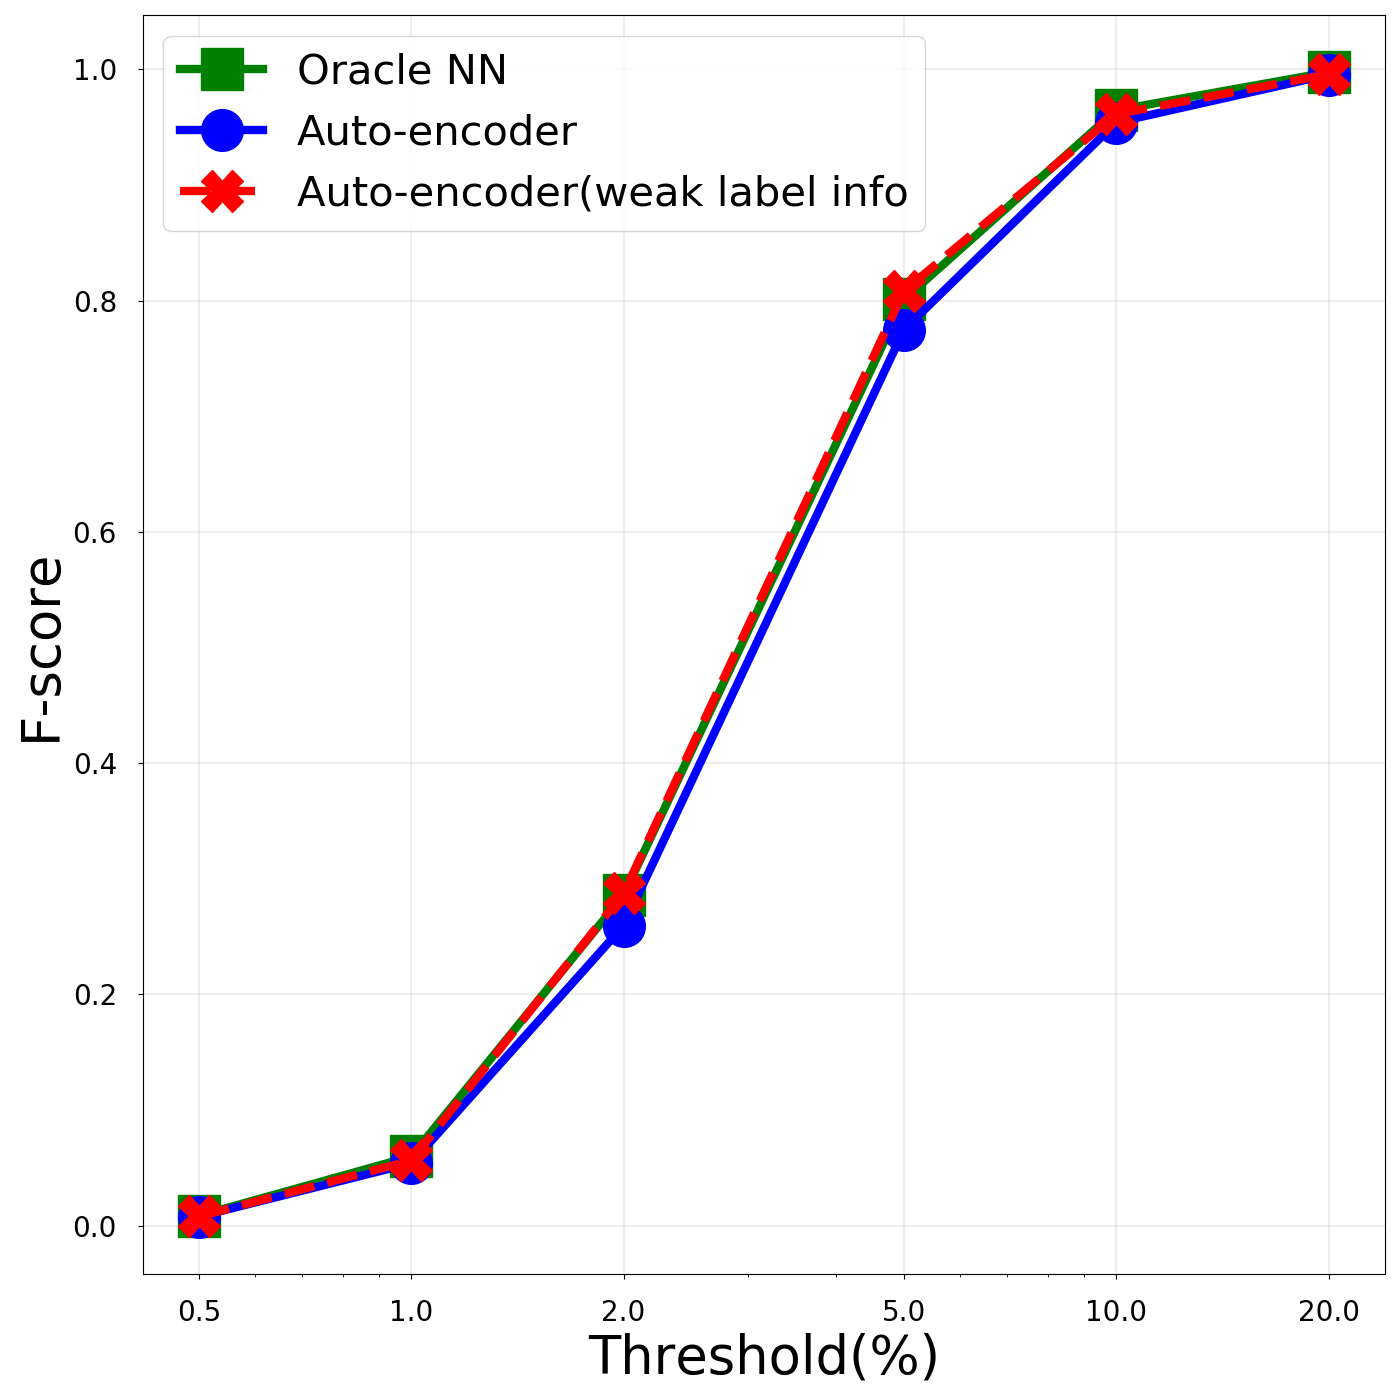
\includegraphics[width=.40\textwidth]{figs/F-compare.png}
    \caption{\small This figure compares the performance of Oracle-NN to that of a standard ResNet auto-encoder based on FoldingNet. These two classifiers achieve almost exactly the same performance, despite the fact that Oracle-NN requires impractical oracle information unavailable during test time.}
    \label{fig:compare-Oracle-NN}
\end{figure}



\begin{figure}
\centering
\begin{tabular}{c@{}}
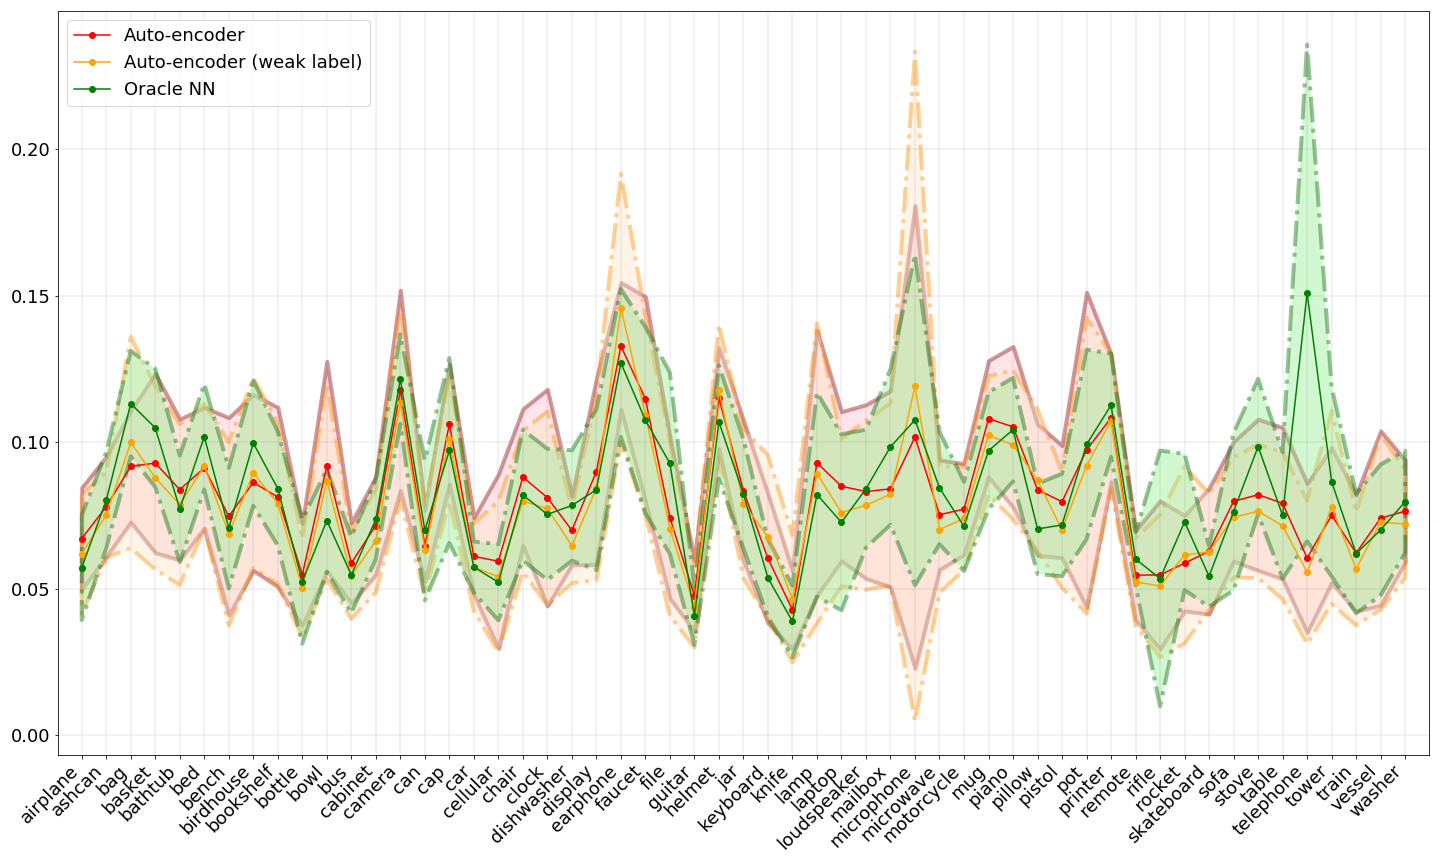
\includegraphics[width=0.99\columnwidth]{figs/CD_per_shape.png} \\
Chamfer Distance \\
\end{tabular}
\caption{Evaluation metrics of reconstruction.  chamfer distance and earth mover's distance per shape. Auto-encoder based methods perform consistently across different classes. }
\label{fig:metric_per_class}
\end{figure}

\begin{figure}[!h]
    \begin{tabular}{c@{}c@{}c@{}c@{}c@{}}
    Input & GT & \makecell[c]{Auto-encoder \\(weak label info)} & Auto-encoder & Oracle NN\\
    	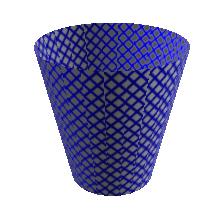
\includegraphics[width=0.11\columnwidth,height=2cm]{figs/real_dataset/Image/ashcan_ff2f13bc0b9d4ade19c52ba9902b5ab0.png} &
    	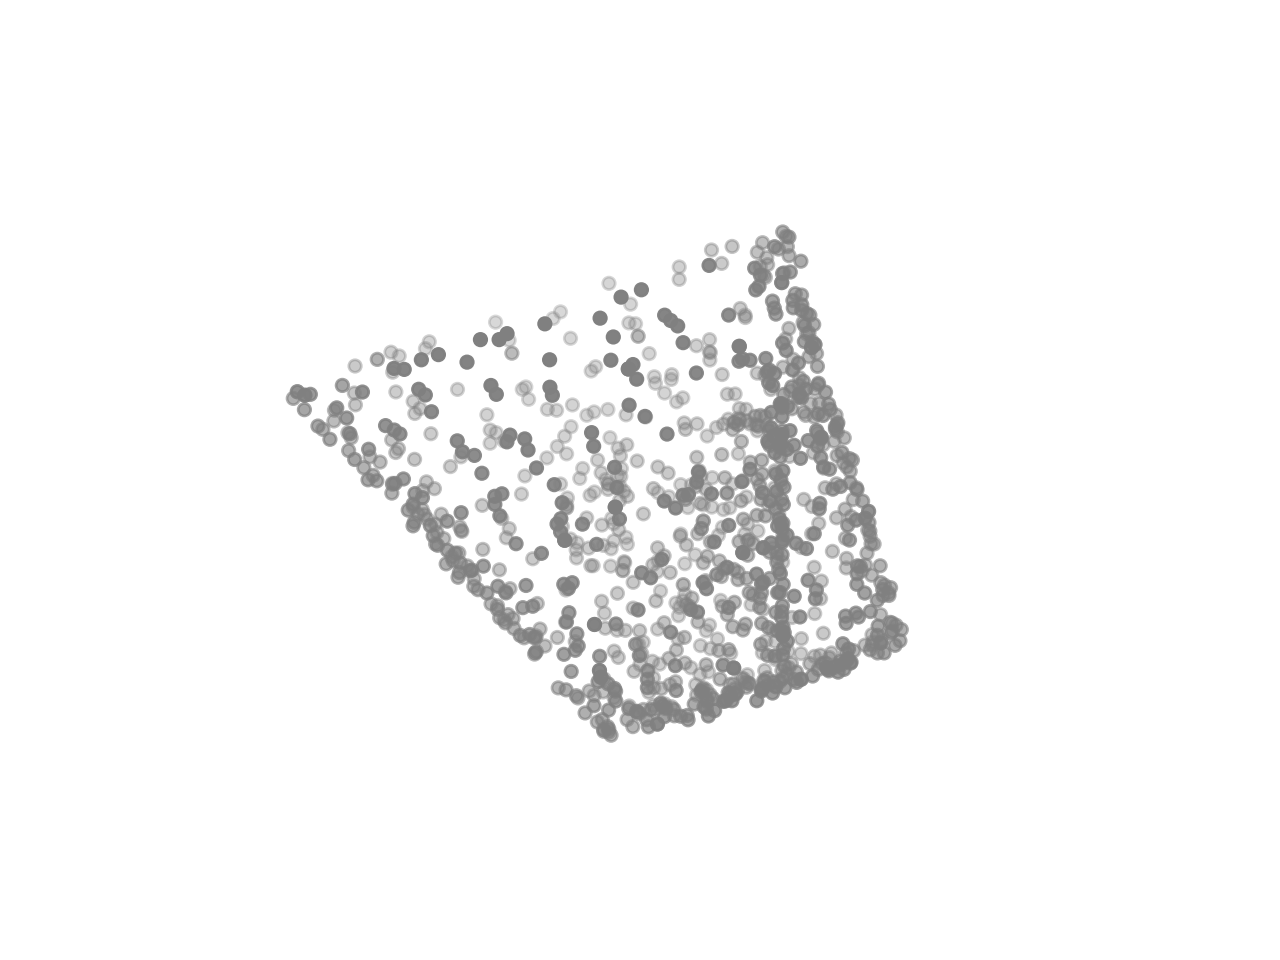
\includegraphics[width=0.22\columnwidth,height=2cm]{figs/real_dataset/GT/ashcan_ff2f13bc0b9d4ade19c52ba9902b5ab0_gt.png} &
    	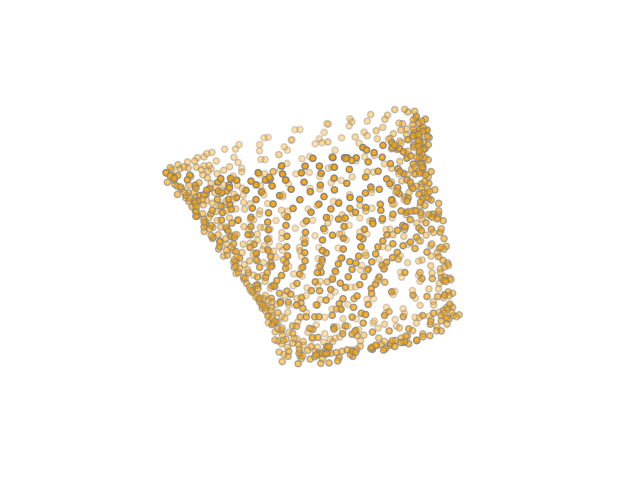
\includegraphics[width=0.22\columnwidth,height=2cm]{figs/real_dataset/AE_label/ashcan_ff2f13bc0b9d4ade19c52ba9902b5ab0_fine.png} &
    	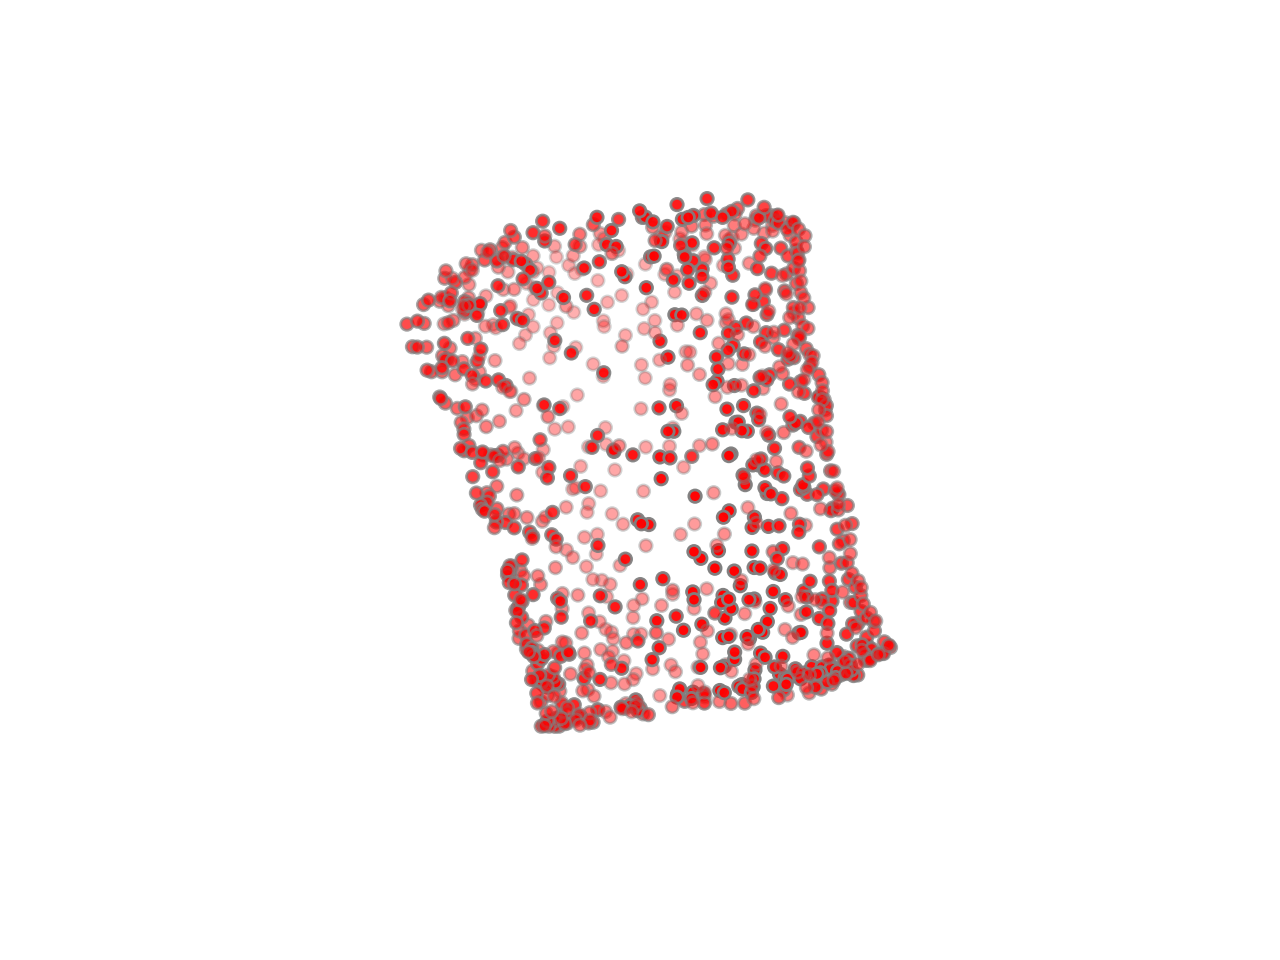
\includegraphics[width=0.22\columnwidth,height=2cm]{figs/real_dataset/AE/ashcan_66d96d2428184442ba6cf6cbb9f4c2bb_fine.png} &
    	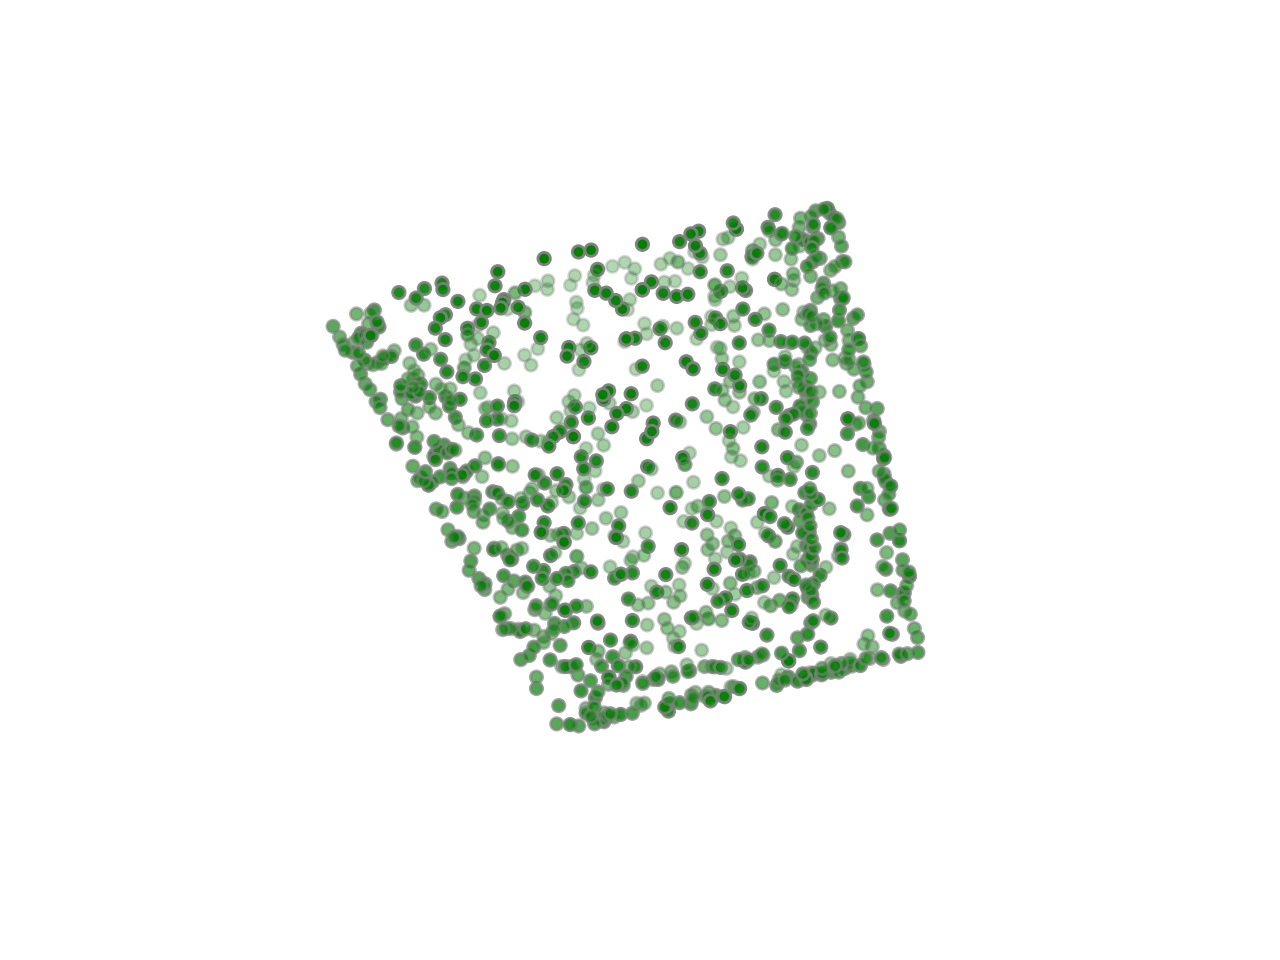
\includegraphics[width=0.22\columnwidth,height=2cm]{figs/real_dataset/oracle/ashcan_ff2f13bc0b9d4ade19c52ba9902b5ab0_oracle.png} \\
    	\vspace{-5mm}
    	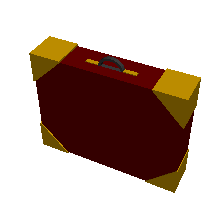
\includegraphics[width=0.11\columnwidth,height=2cm]{figs/real_dataset/Image/bag_8569a0c606bbba73d9985ad45fbb635e.png} &
    	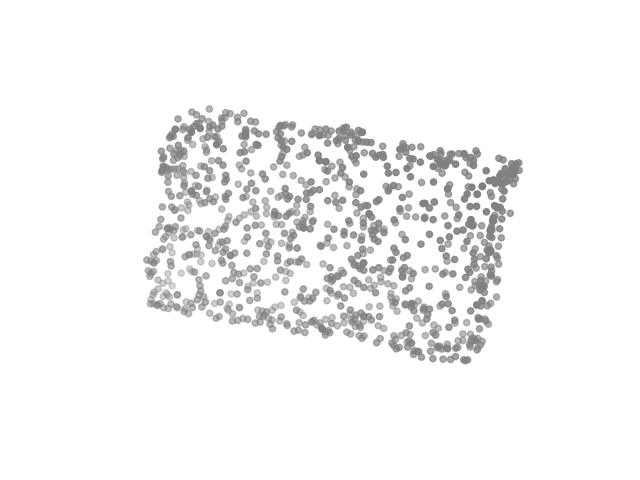
\includegraphics[width=0.22\columnwidth,height=2cm]{figs/real_dataset/GT/bag_8569a0c606bbba73d9985ad45fbb635e.png} &
    	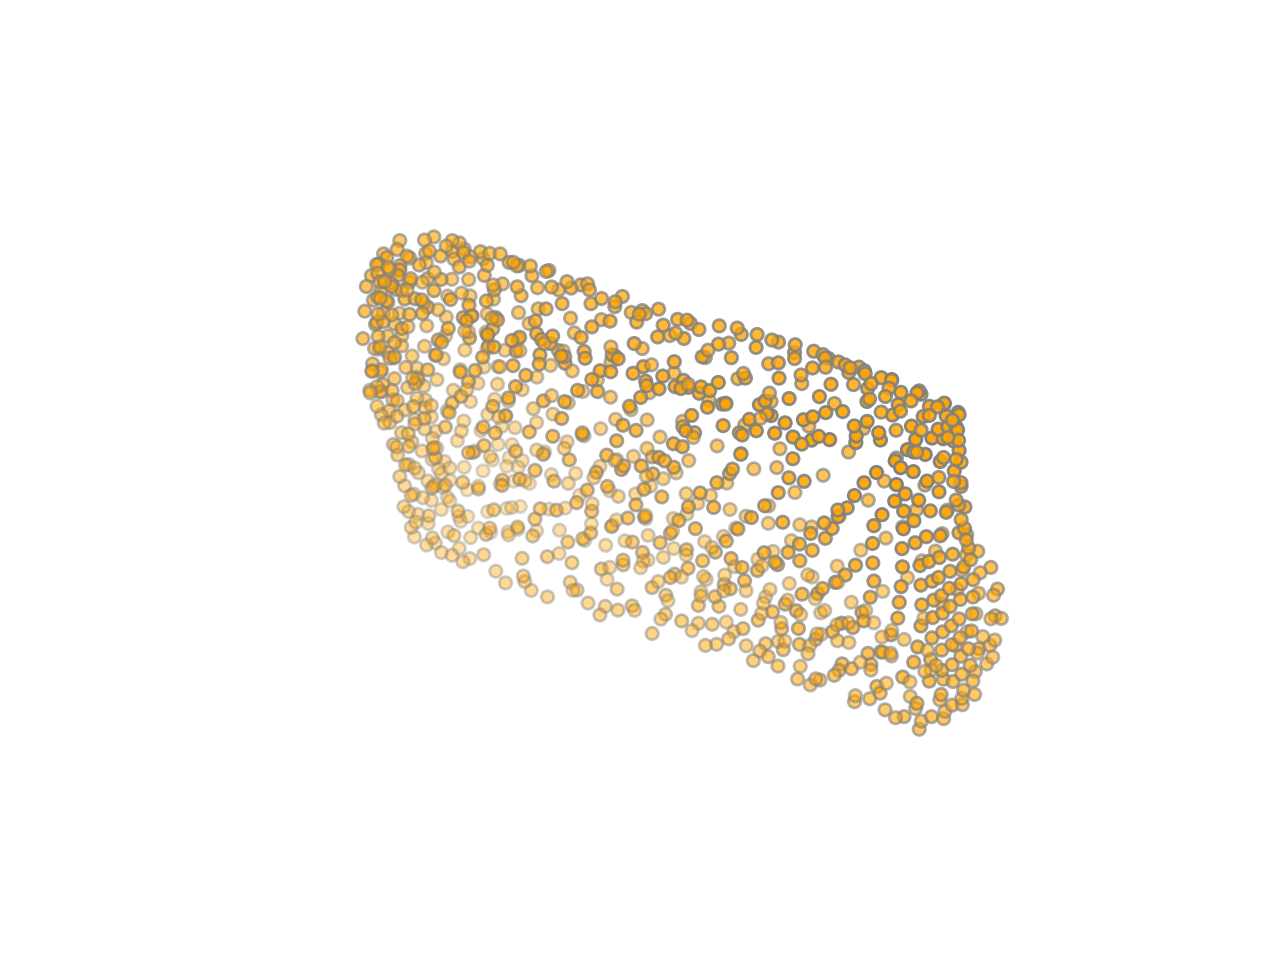
\includegraphics[width=0.22\columnwidth,height=2cm]{figs/real_dataset/AE_label/bag_8569a0c606bbba73d9985ad45fbb635e_fine.png} &
    	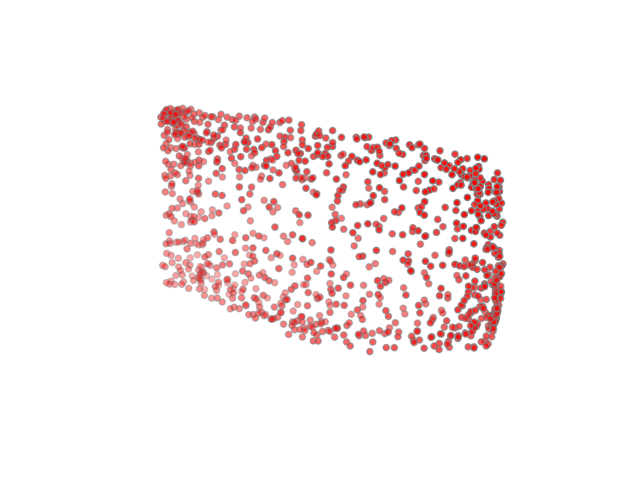
\includegraphics[width=0.22\columnwidth,height=2cm]{figs/real_dataset/AE/bag_8569a0c606bbba73d9985ad45fbb635e.png} &
    	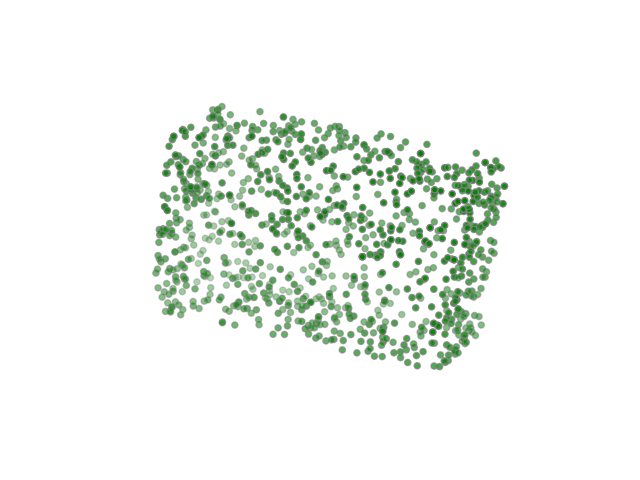
\includegraphics[width=0.22\columnwidth,height=2cm]{figs/real_dataset/oracle/bag_8569a0c606bbba73d9985ad45fbb635e.png} \\  
    	\vspace{-5mm}
    	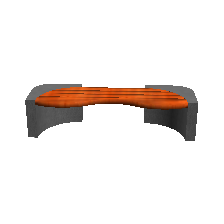
\includegraphics[width=0.11\columnwidth,height=2cm]{figs/real_dataset/Image/bench_17ebf60b6ba61ae949e6f7df978f3373.png} &
    	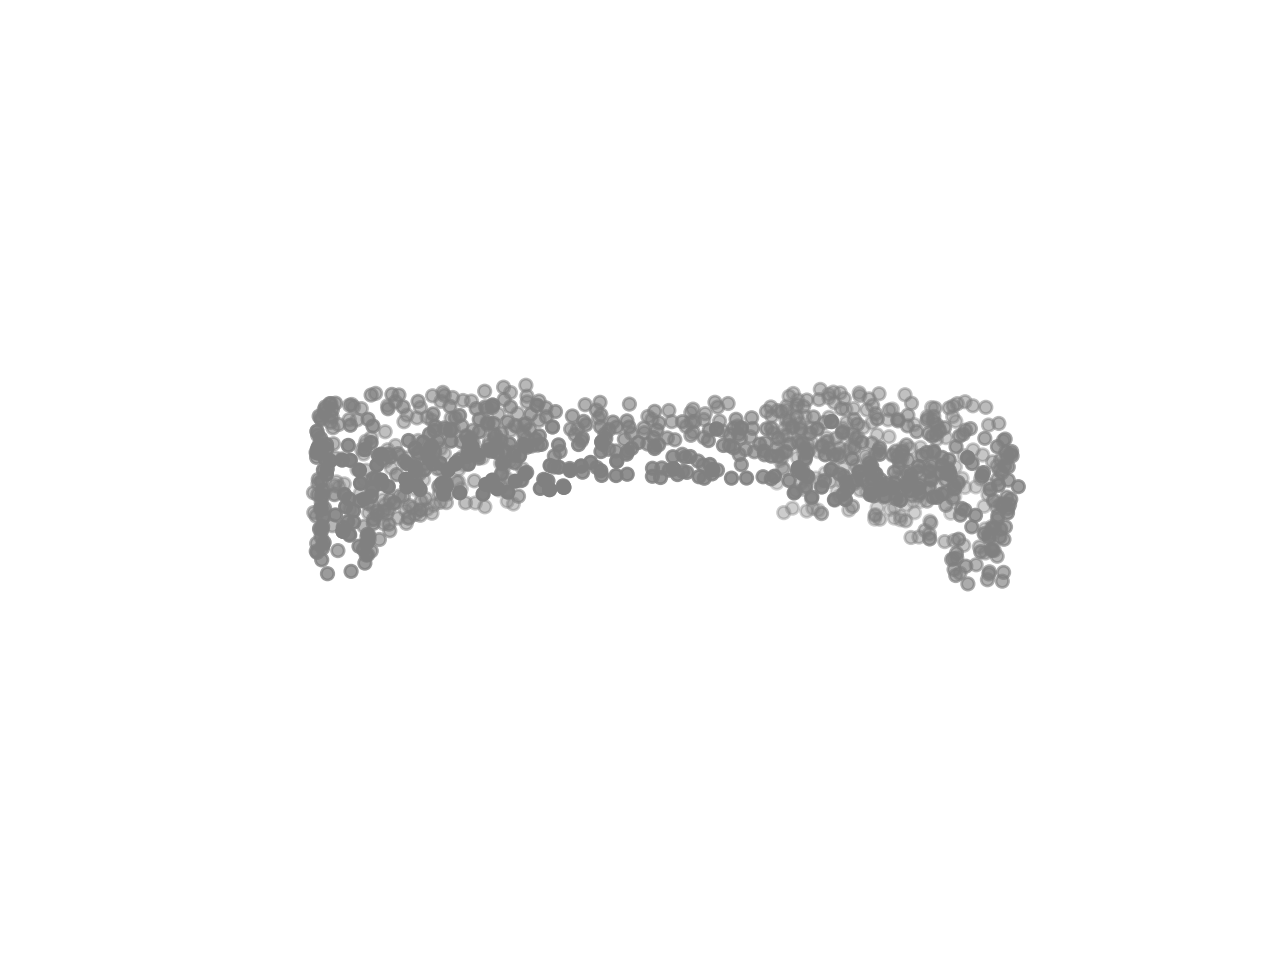
\includegraphics[width=0.22\columnwidth,height=2cm]{figs/real_dataset/GT/bench_17ebf60b6ba61ae949e6f7df978f3373_gt.png} &
    	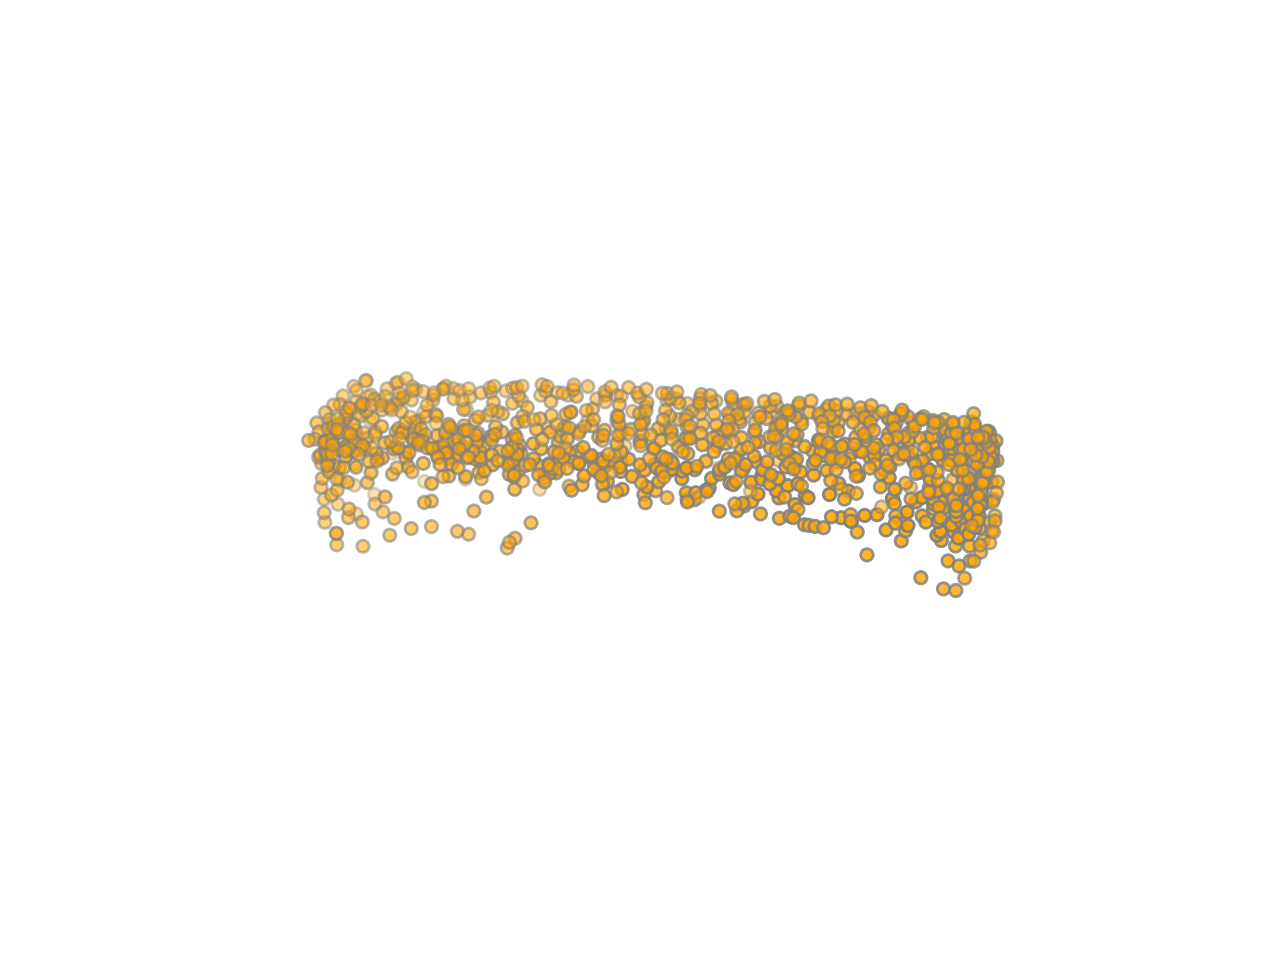
\includegraphics[width=0.22\columnwidth,height=2cm]{figs/real_dataset/AE_label/bench_17ebf60b6ba61ae949e6f7df978f3373_fine.png} &
    	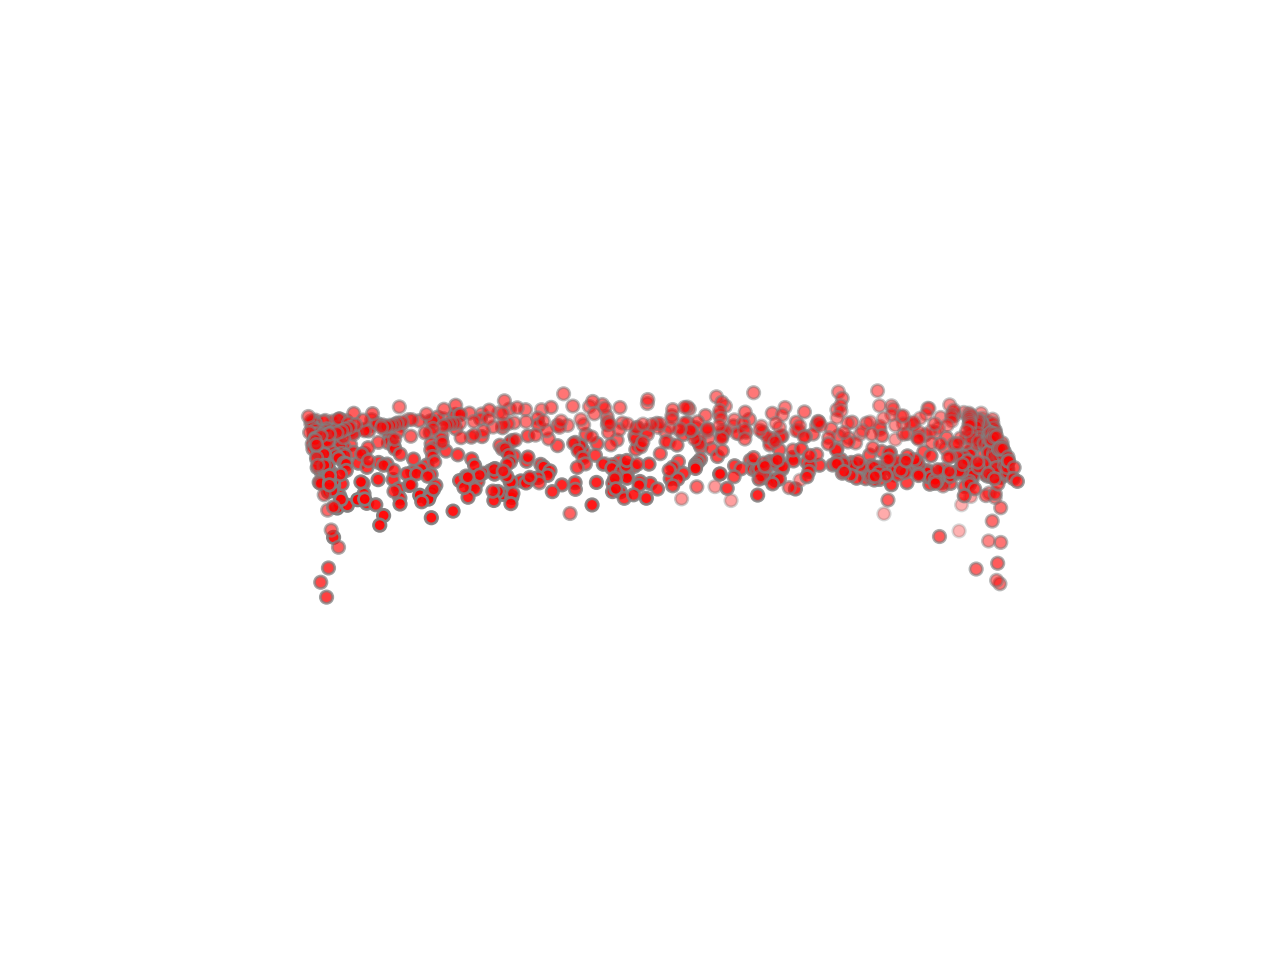
\includegraphics[width=0.22\columnwidth,height=2cm]{figs/real_dataset/AE/bench_17ebf60b6ba61ae949e6f7df978f3373_fine.png} &
    	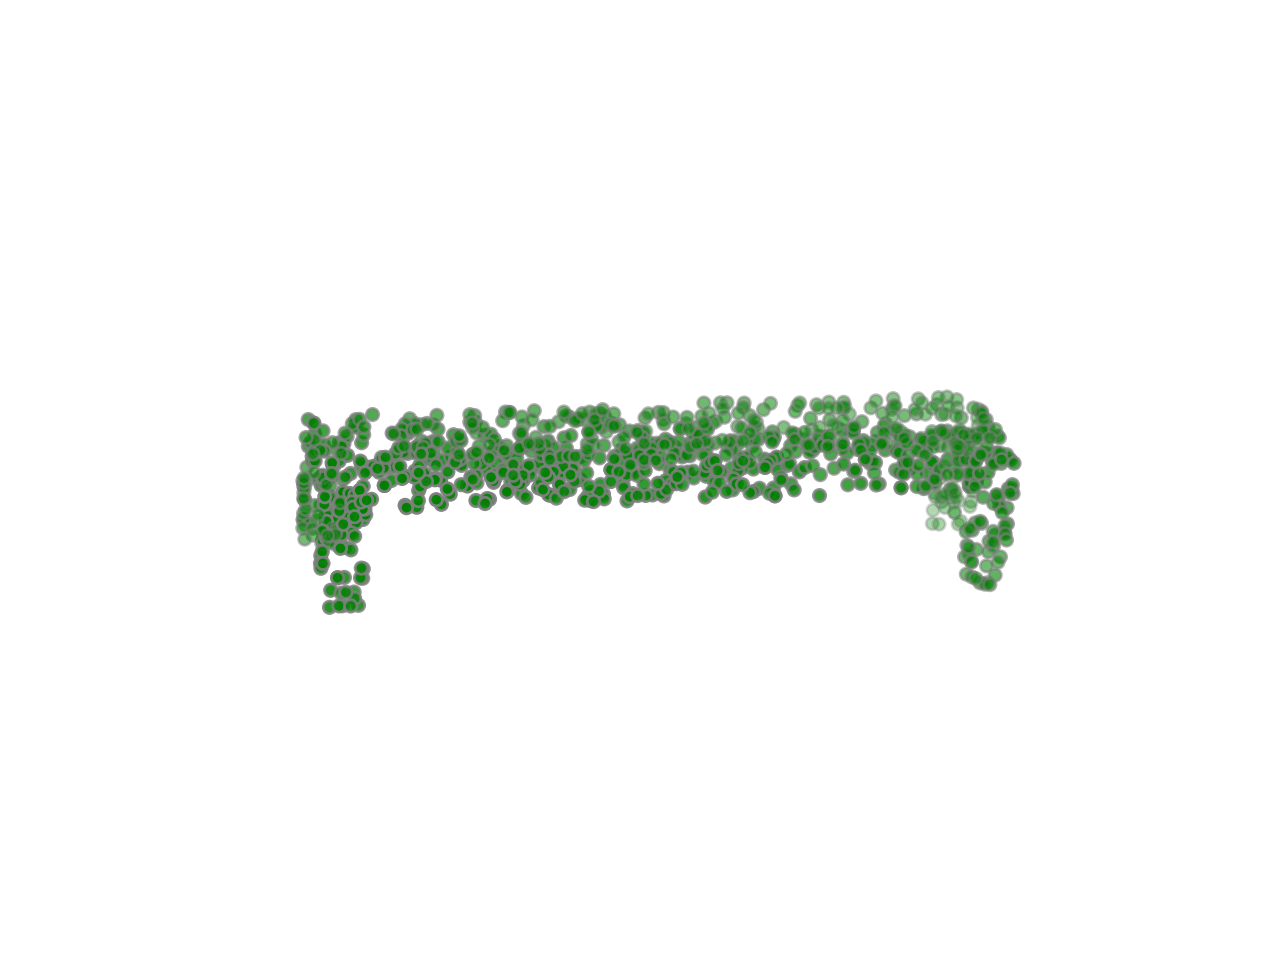
\includegraphics[width=0.22\columnwidth,height=2cm]{figs/real_dataset/oracle/bench_17ebf60b6ba61ae949e6f7df978f3373_oracle.png} \\
    	\vspace{-5mm}
    	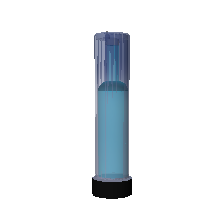
\includegraphics[width=0.11\columnwidth,height=2cm]{figs/real_dataset/Image/bottle_ab3795042c759b6798646029ad91cbbd.png} &
    	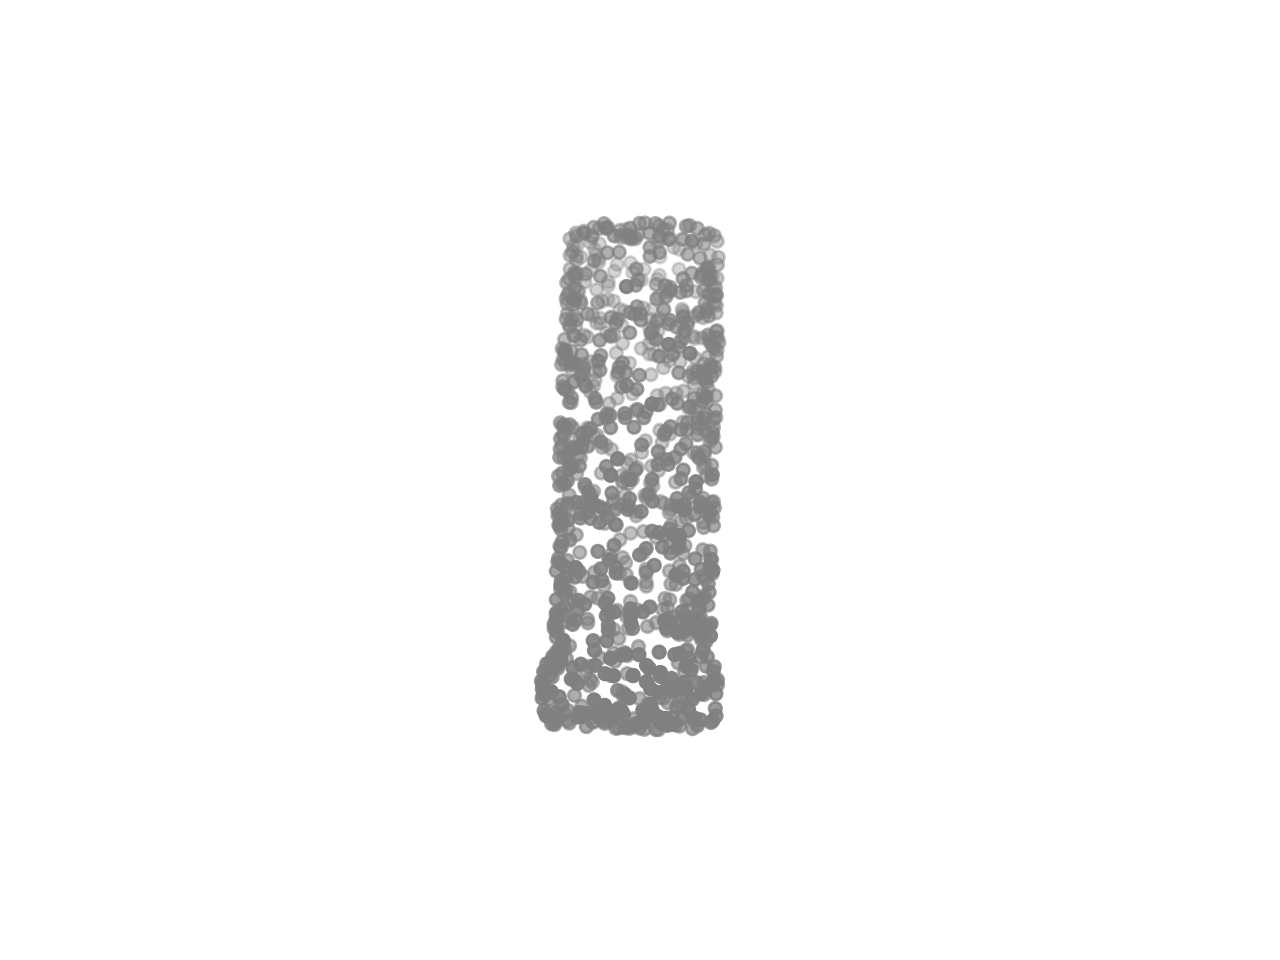
\includegraphics[width=0.22\columnwidth,height=2cm]{figs/real_dataset/GT/bottle_ab3795042c759b6798646029ad91cbbd_gt.png} &
    	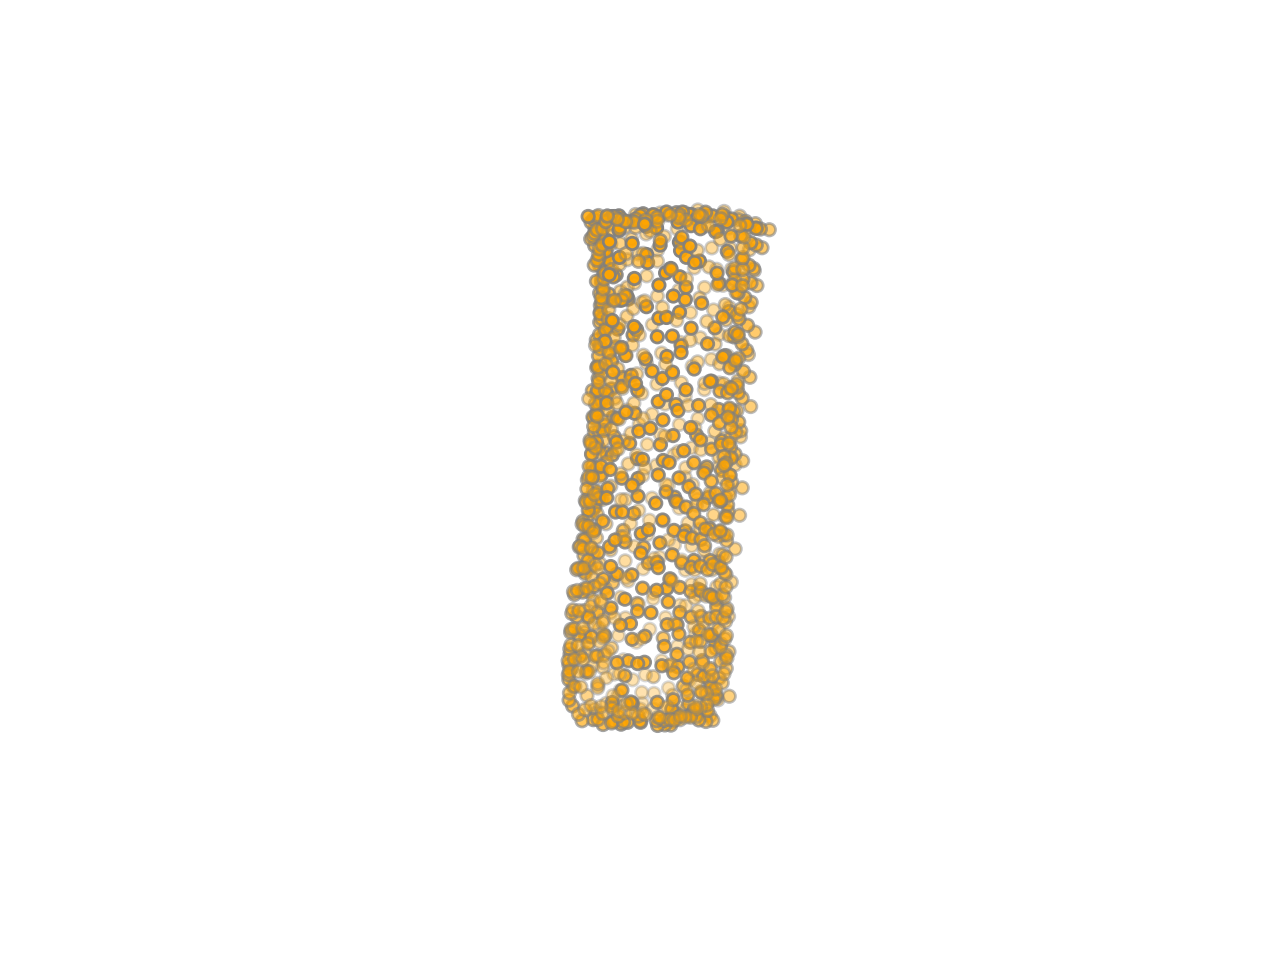
\includegraphics[width=0.22\columnwidth,height=2cm]{figs/real_dataset/AE_label/bottle_ab3795042c759b6798646029ad91cbbd_fine.png} &
    	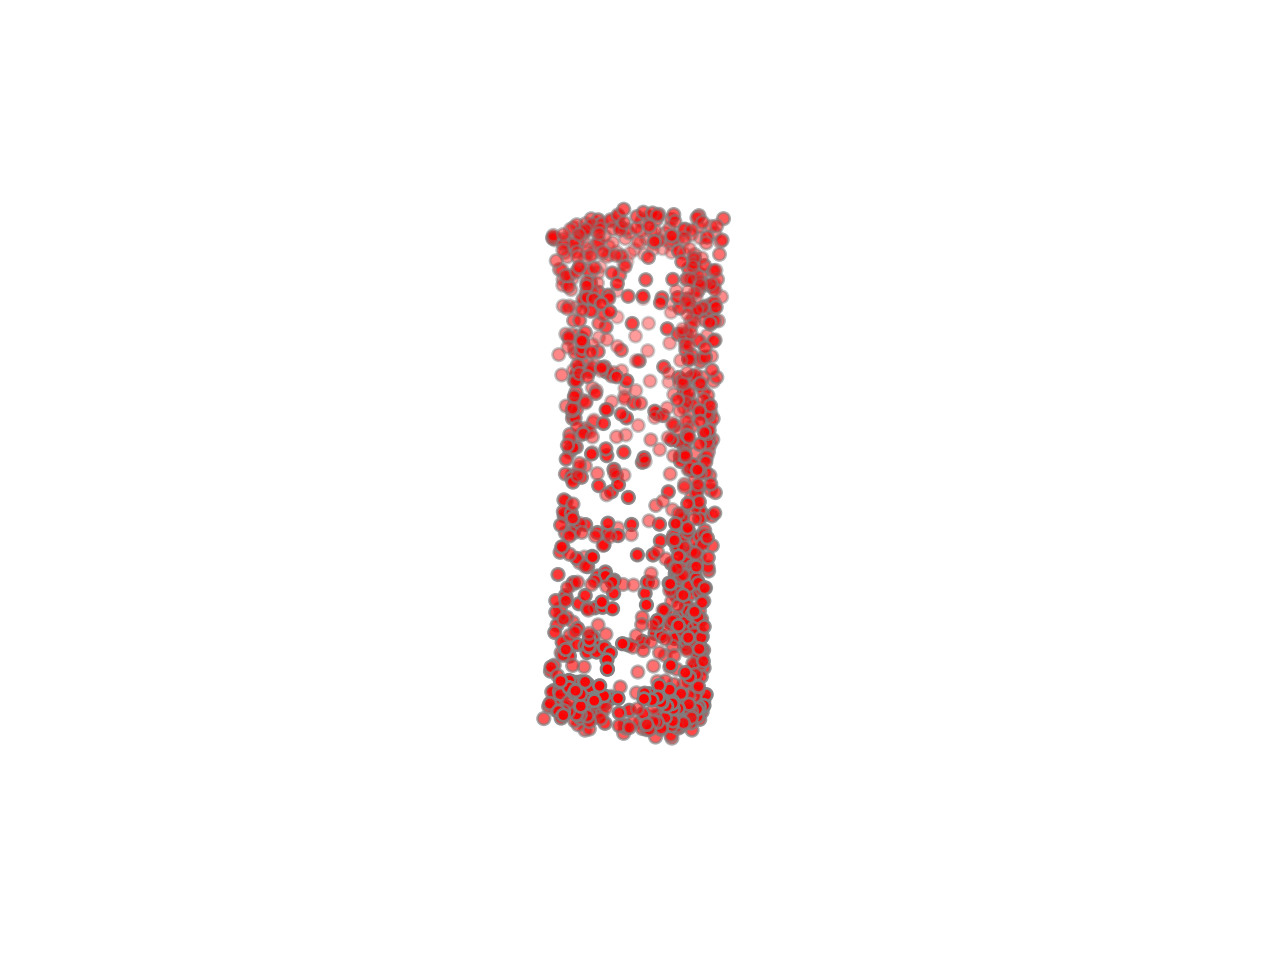
\includegraphics[width=0.22\columnwidth,height=2cm]{figs/real_dataset/AE/bottle_ab3795042c759b6798646029ad91cbbd_fine.png} &
    	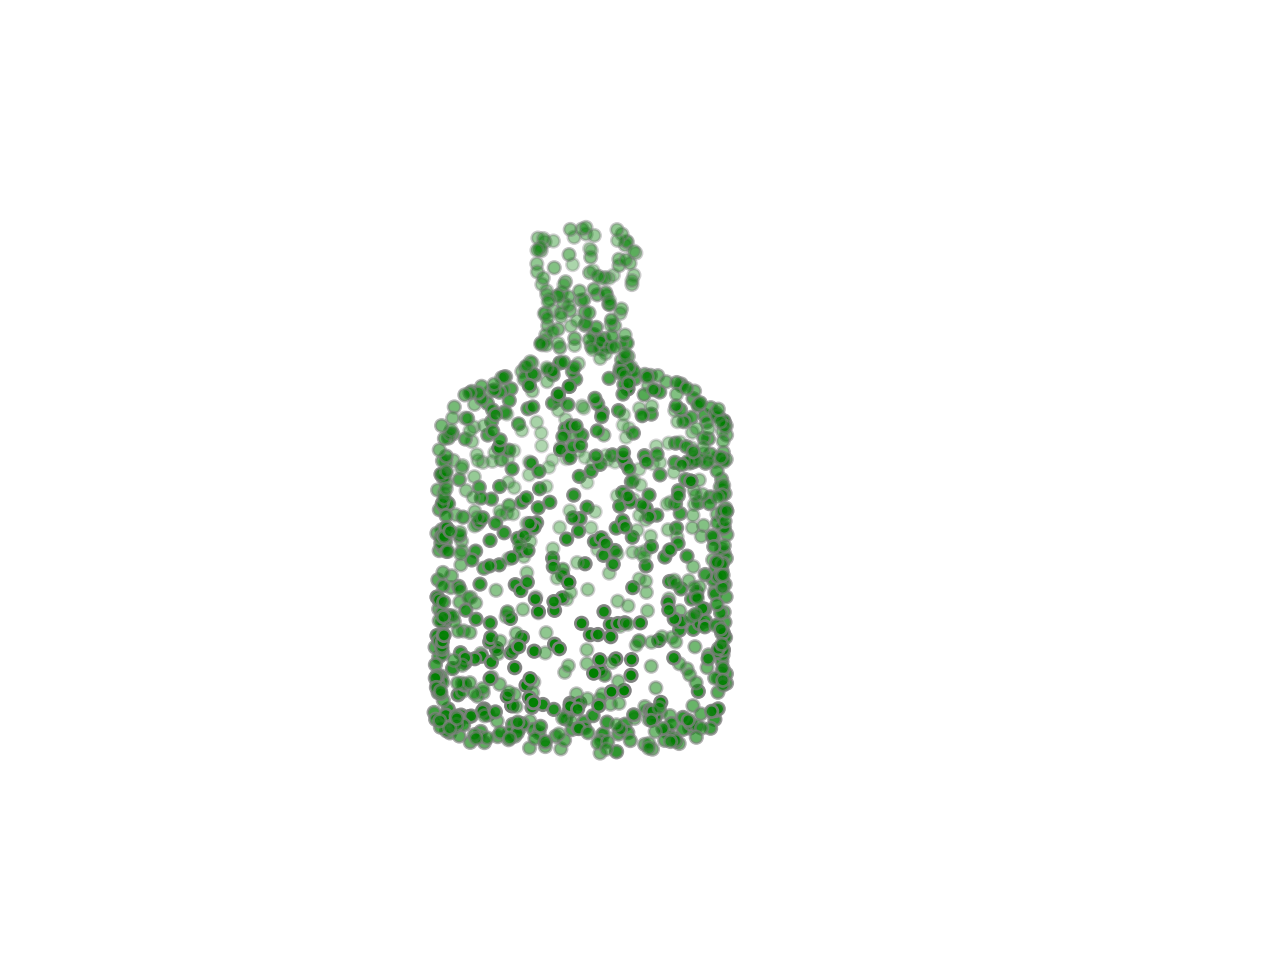
\includegraphics[width=0.22\columnwidth,height=2cm]{figs/real_dataset/oracle/bottle_3b956918a41da89c325e6e8eb2c67fd8_oracle.png} \\
    	\vspace{-5mm}
    	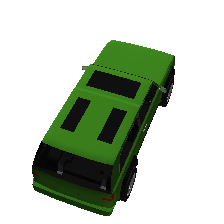
\includegraphics[width=0.11\columnwidth,height=2cm]{figs/real_dataset/Image/car_8b049c92888475f67c3c6f82a395b347.png} &
    	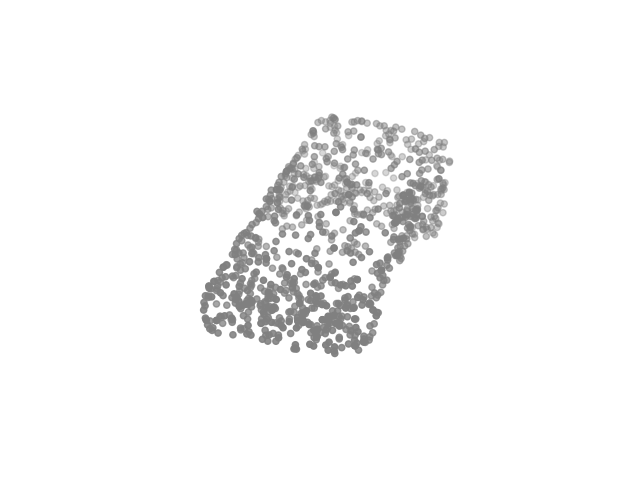
\includegraphics[width=0.22\columnwidth,height=2cm]{figs/real_dataset/GT/car_8b049c92888475f67c3c6f82a395b347.png} &
    	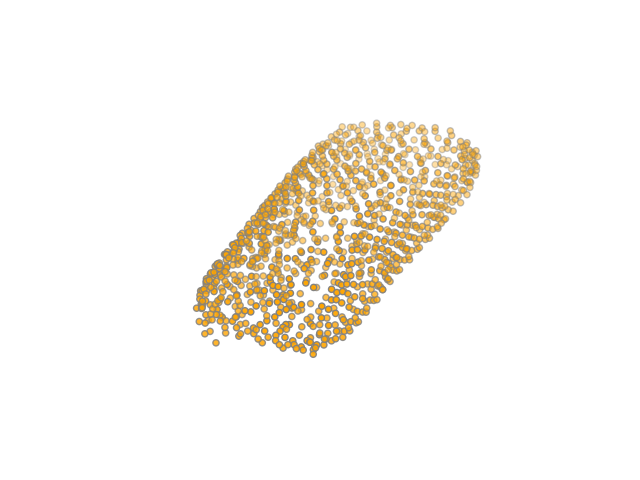
\includegraphics[width=0.22\columnwidth,height=2cm]{figs/real_dataset/AE_label/car_8b049c92888475f67c3c6f82a395b347_fine.png} &
    	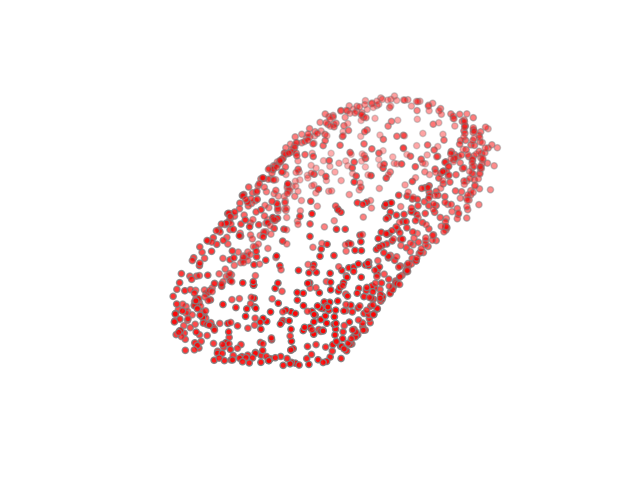
\includegraphics[width=0.22\columnwidth,height=2cm]{figs/real_dataset/AE/car_8b049c92888475f67c3c6f82a395b347.png} &
    	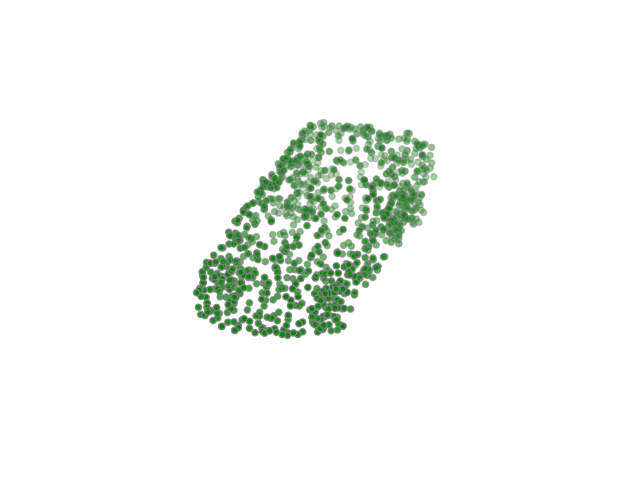
\includegraphics[width=0.22\columnwidth,height=2cm]{figs/real_dataset/oracle/car_8b049c92888475f67c3c6f82a395b347.png} \\
    	\vspace{-5mm}
    	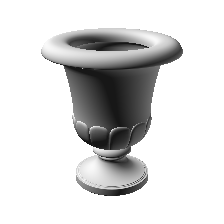
\includegraphics[width=0.11\columnwidth,height=2cm]{figs/real_dataset/Image/jar_d56098d4d83f5976a2c59a4d90e63212.png} &
    	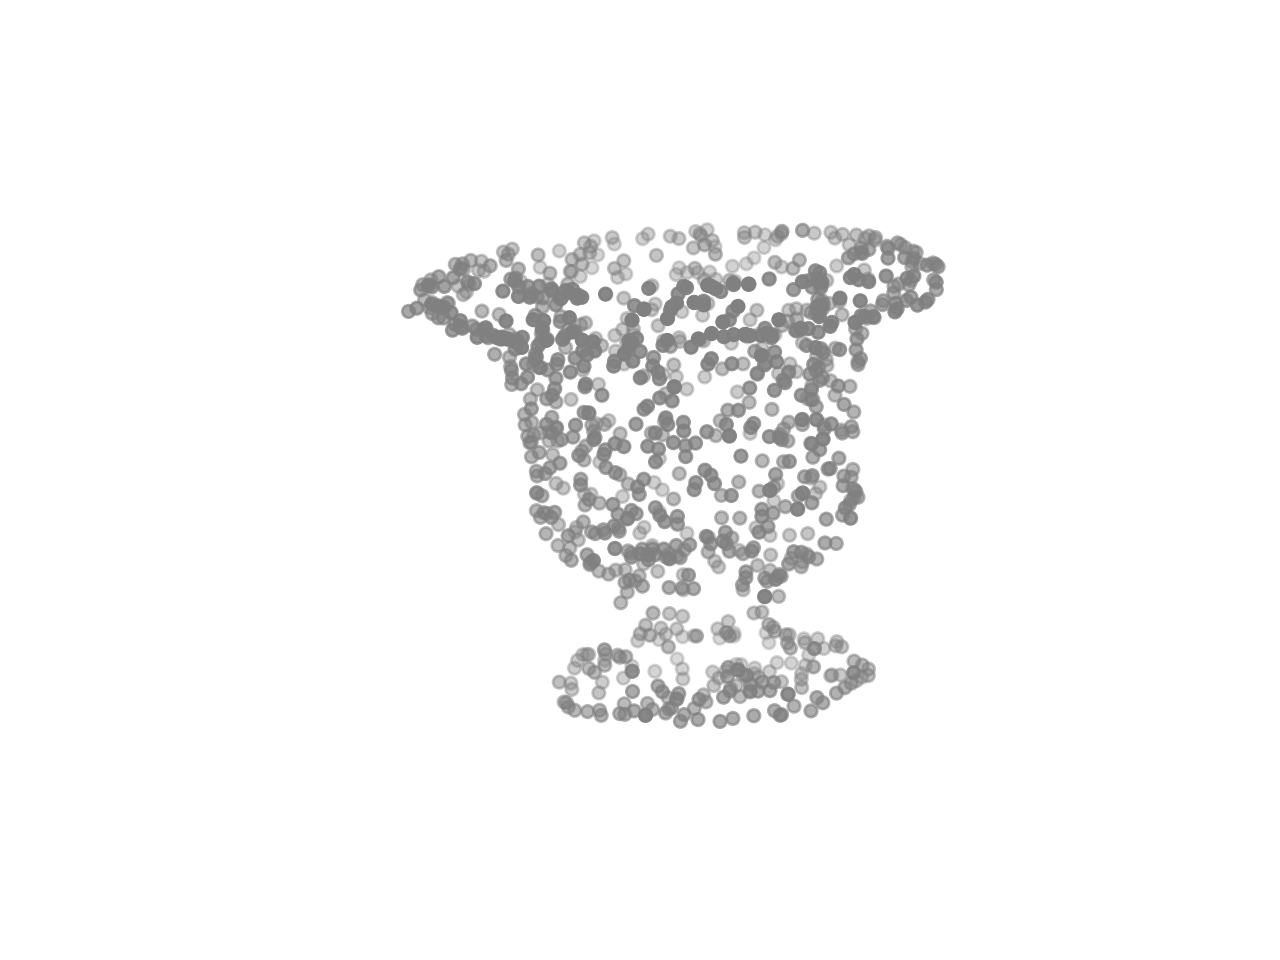
\includegraphics[width=0.22\columnwidth,height=2cm]{figs/real_dataset/GT/jar_d56098d4d83f5976a2c59a4d90e63212_gt.png} &
    	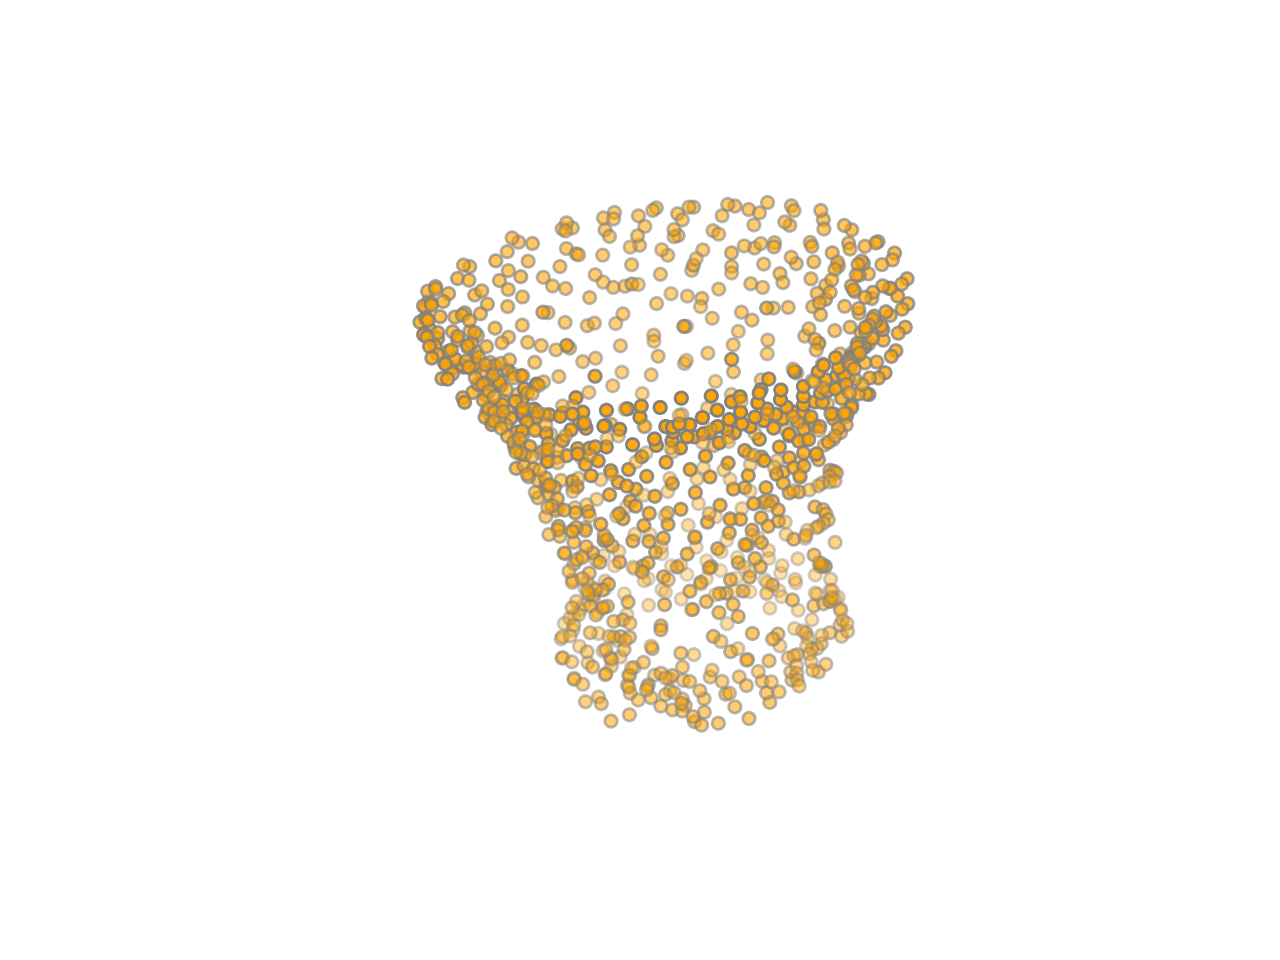
\includegraphics[width=0.22\columnwidth,height=2cm]{figs/real_dataset/AE_label/jar_d56098d4d83f5976a2c59a4d90e63212_fine.png} &
    	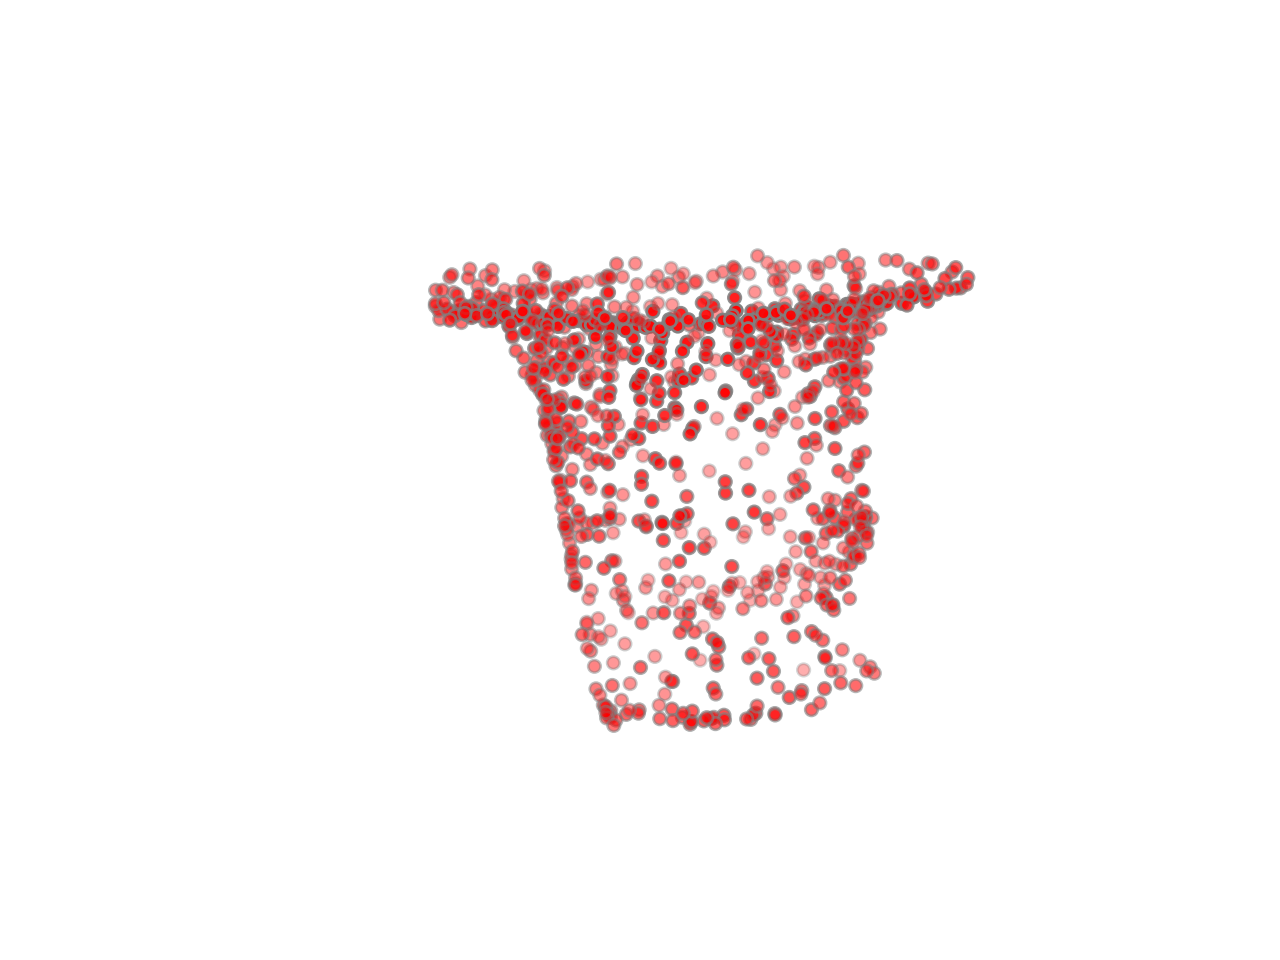
\includegraphics[width=0.22\columnwidth,height=2cm]{figs/real_dataset/AE/jar_d56098d4d83f5976a2c59a4d90e63212_fine.png} &
    	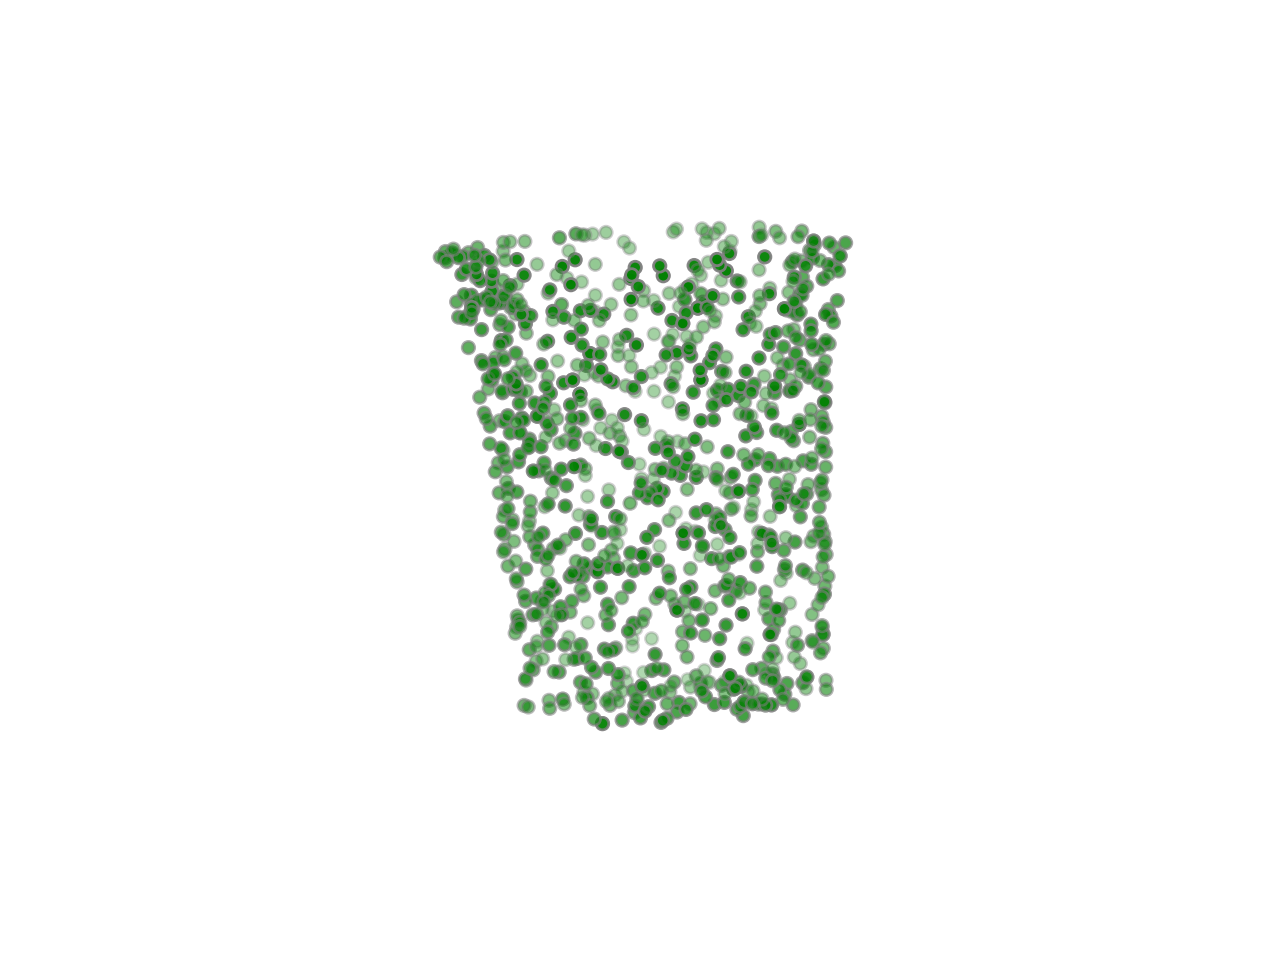
\includegraphics[width=0.22\columnwidth,height=2cm]{figs/real_dataset/oracle/jar_d56098d4d83f5976a2c59a4d90e63212_oracle.png}
    	\\
    \end{tabular}
    \caption{\small Qualitative results show that standard auto-encoders achieve comparable reconstruction performance to Oracle-NN. }
    \label{fig:visualize_KC}
\end{figure}

\FloatBarrier
\subsubsection{机制探究}
\begin{figure}
	\begin{subfigure}[t]{0.3\linewidth} \centering 
     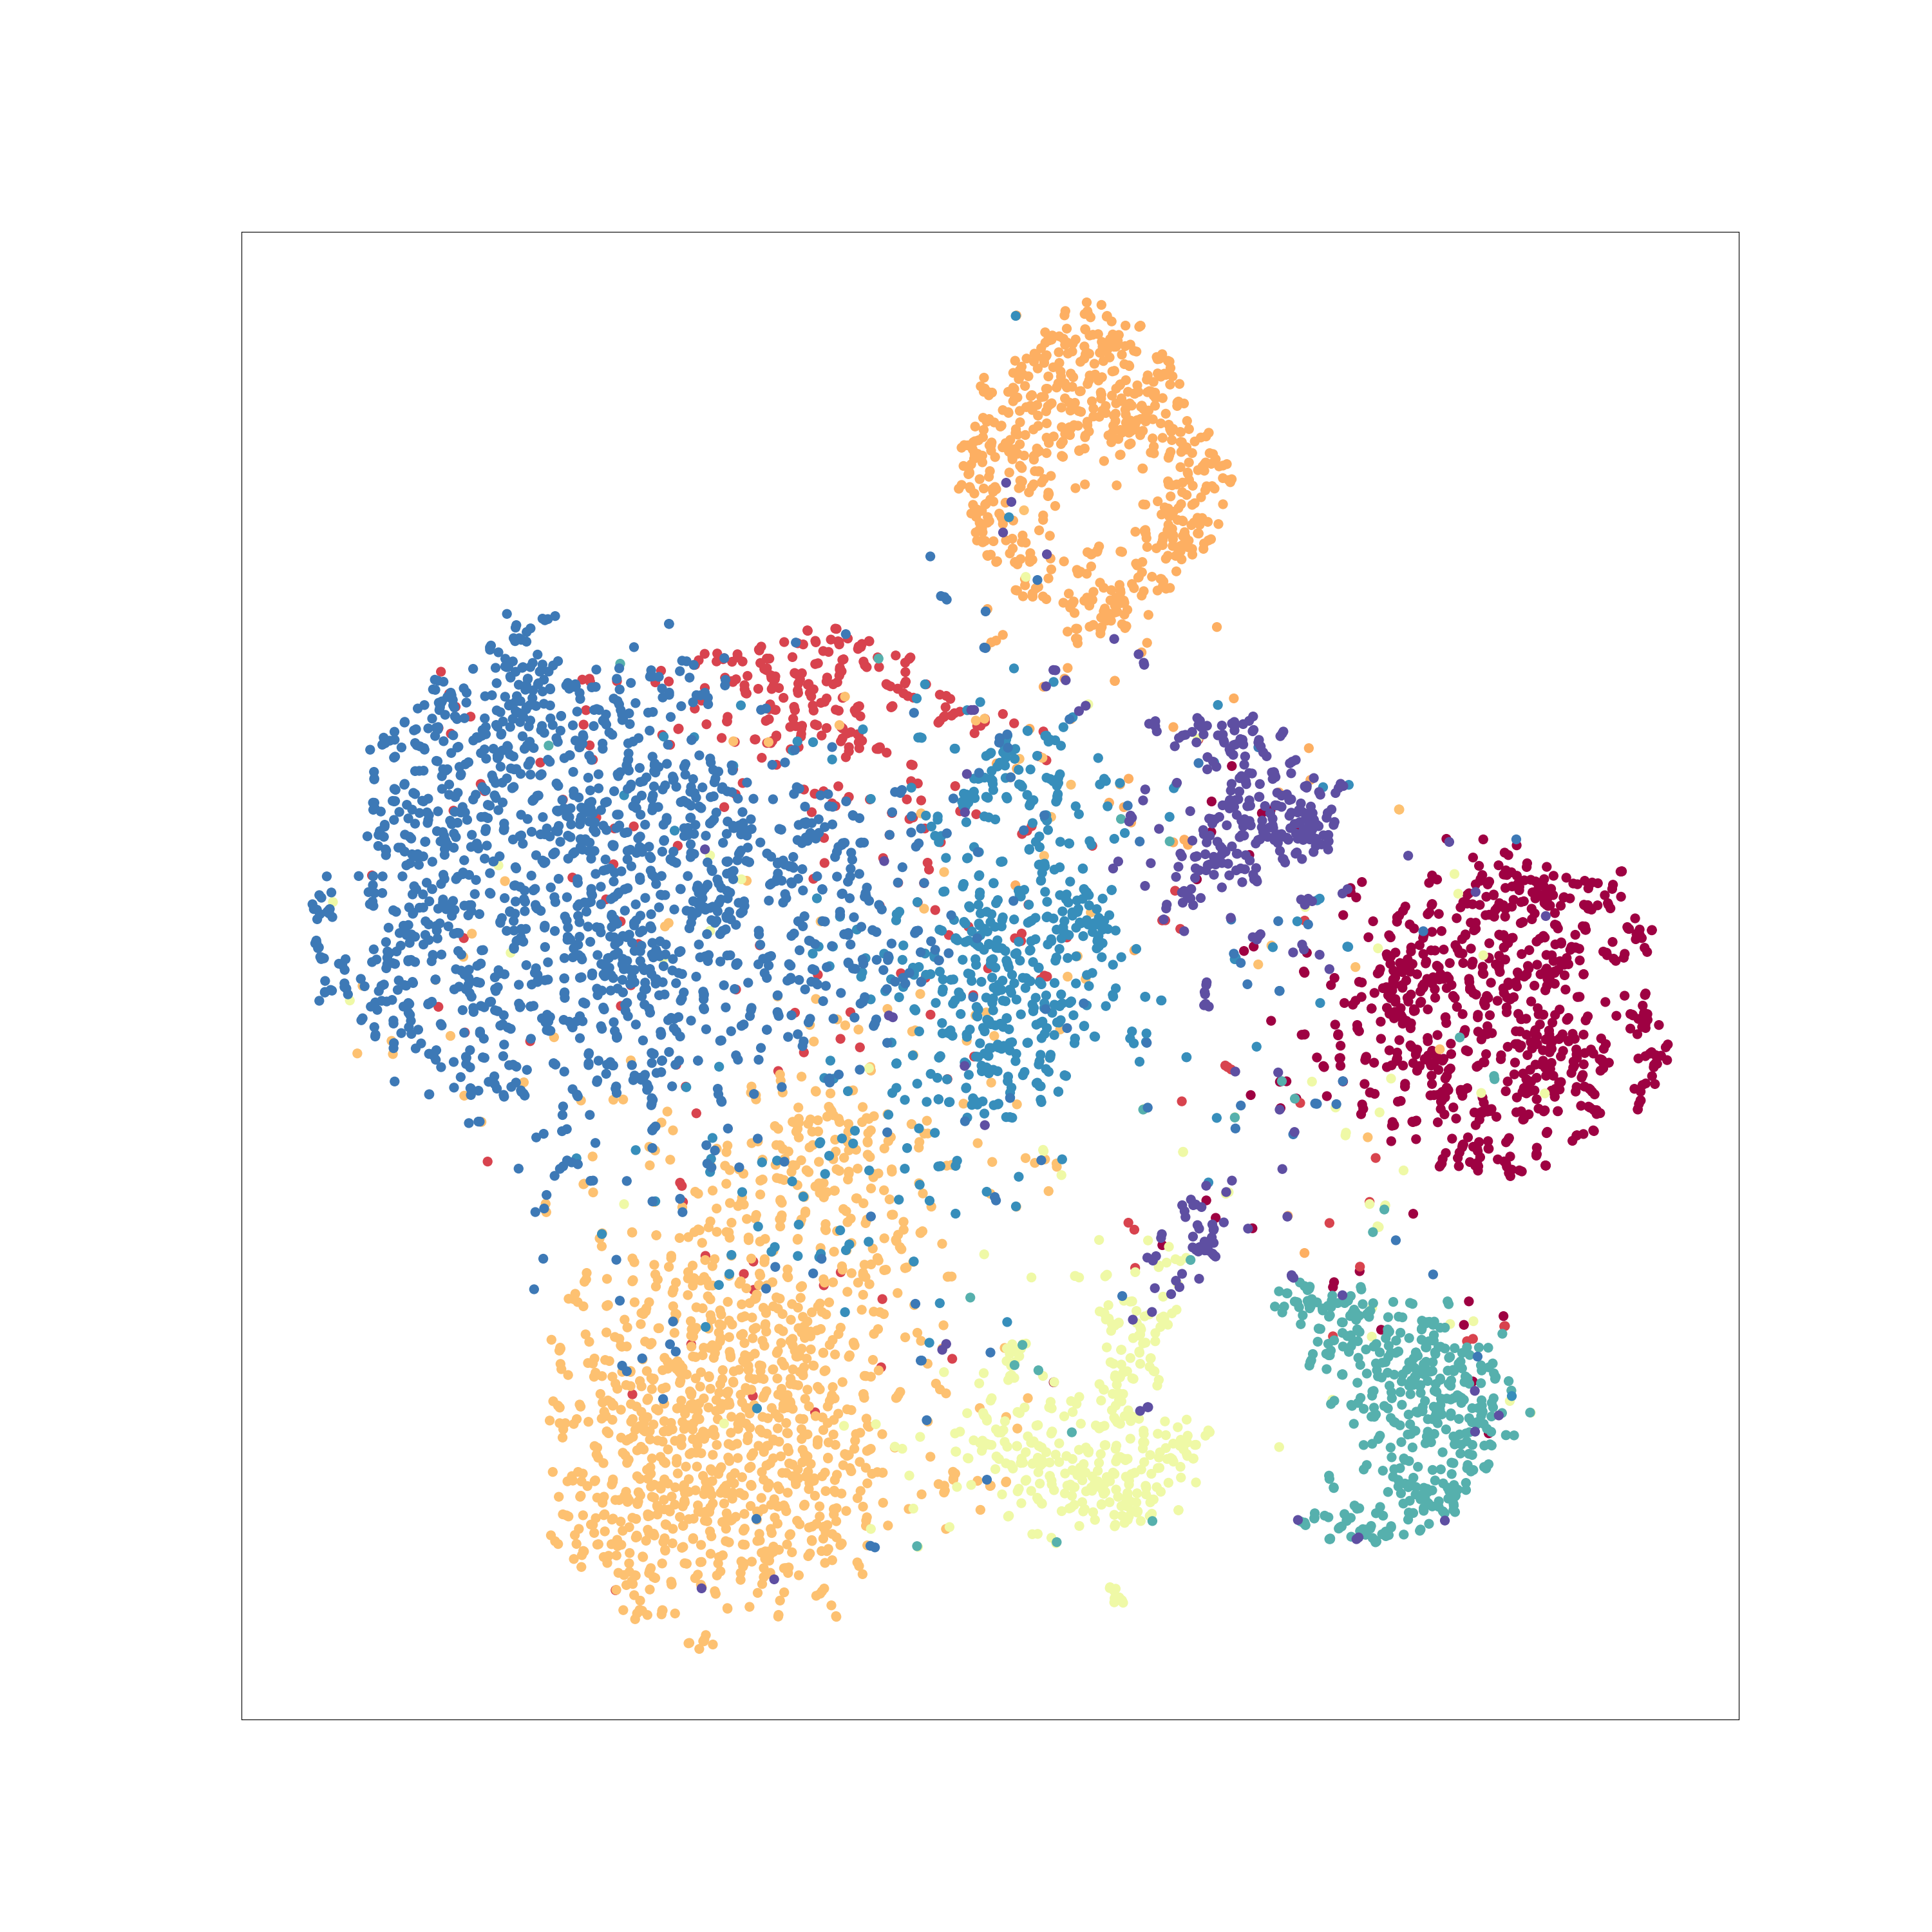
\includegraphics[width=\columnwidth]{figs/T-SNE-class.png}
     \caption{With labels}\label{fig:T-SNE1}
   \end{subfigure}
   \begin{subfigure}[t]{0.3\linewidth} \centering
    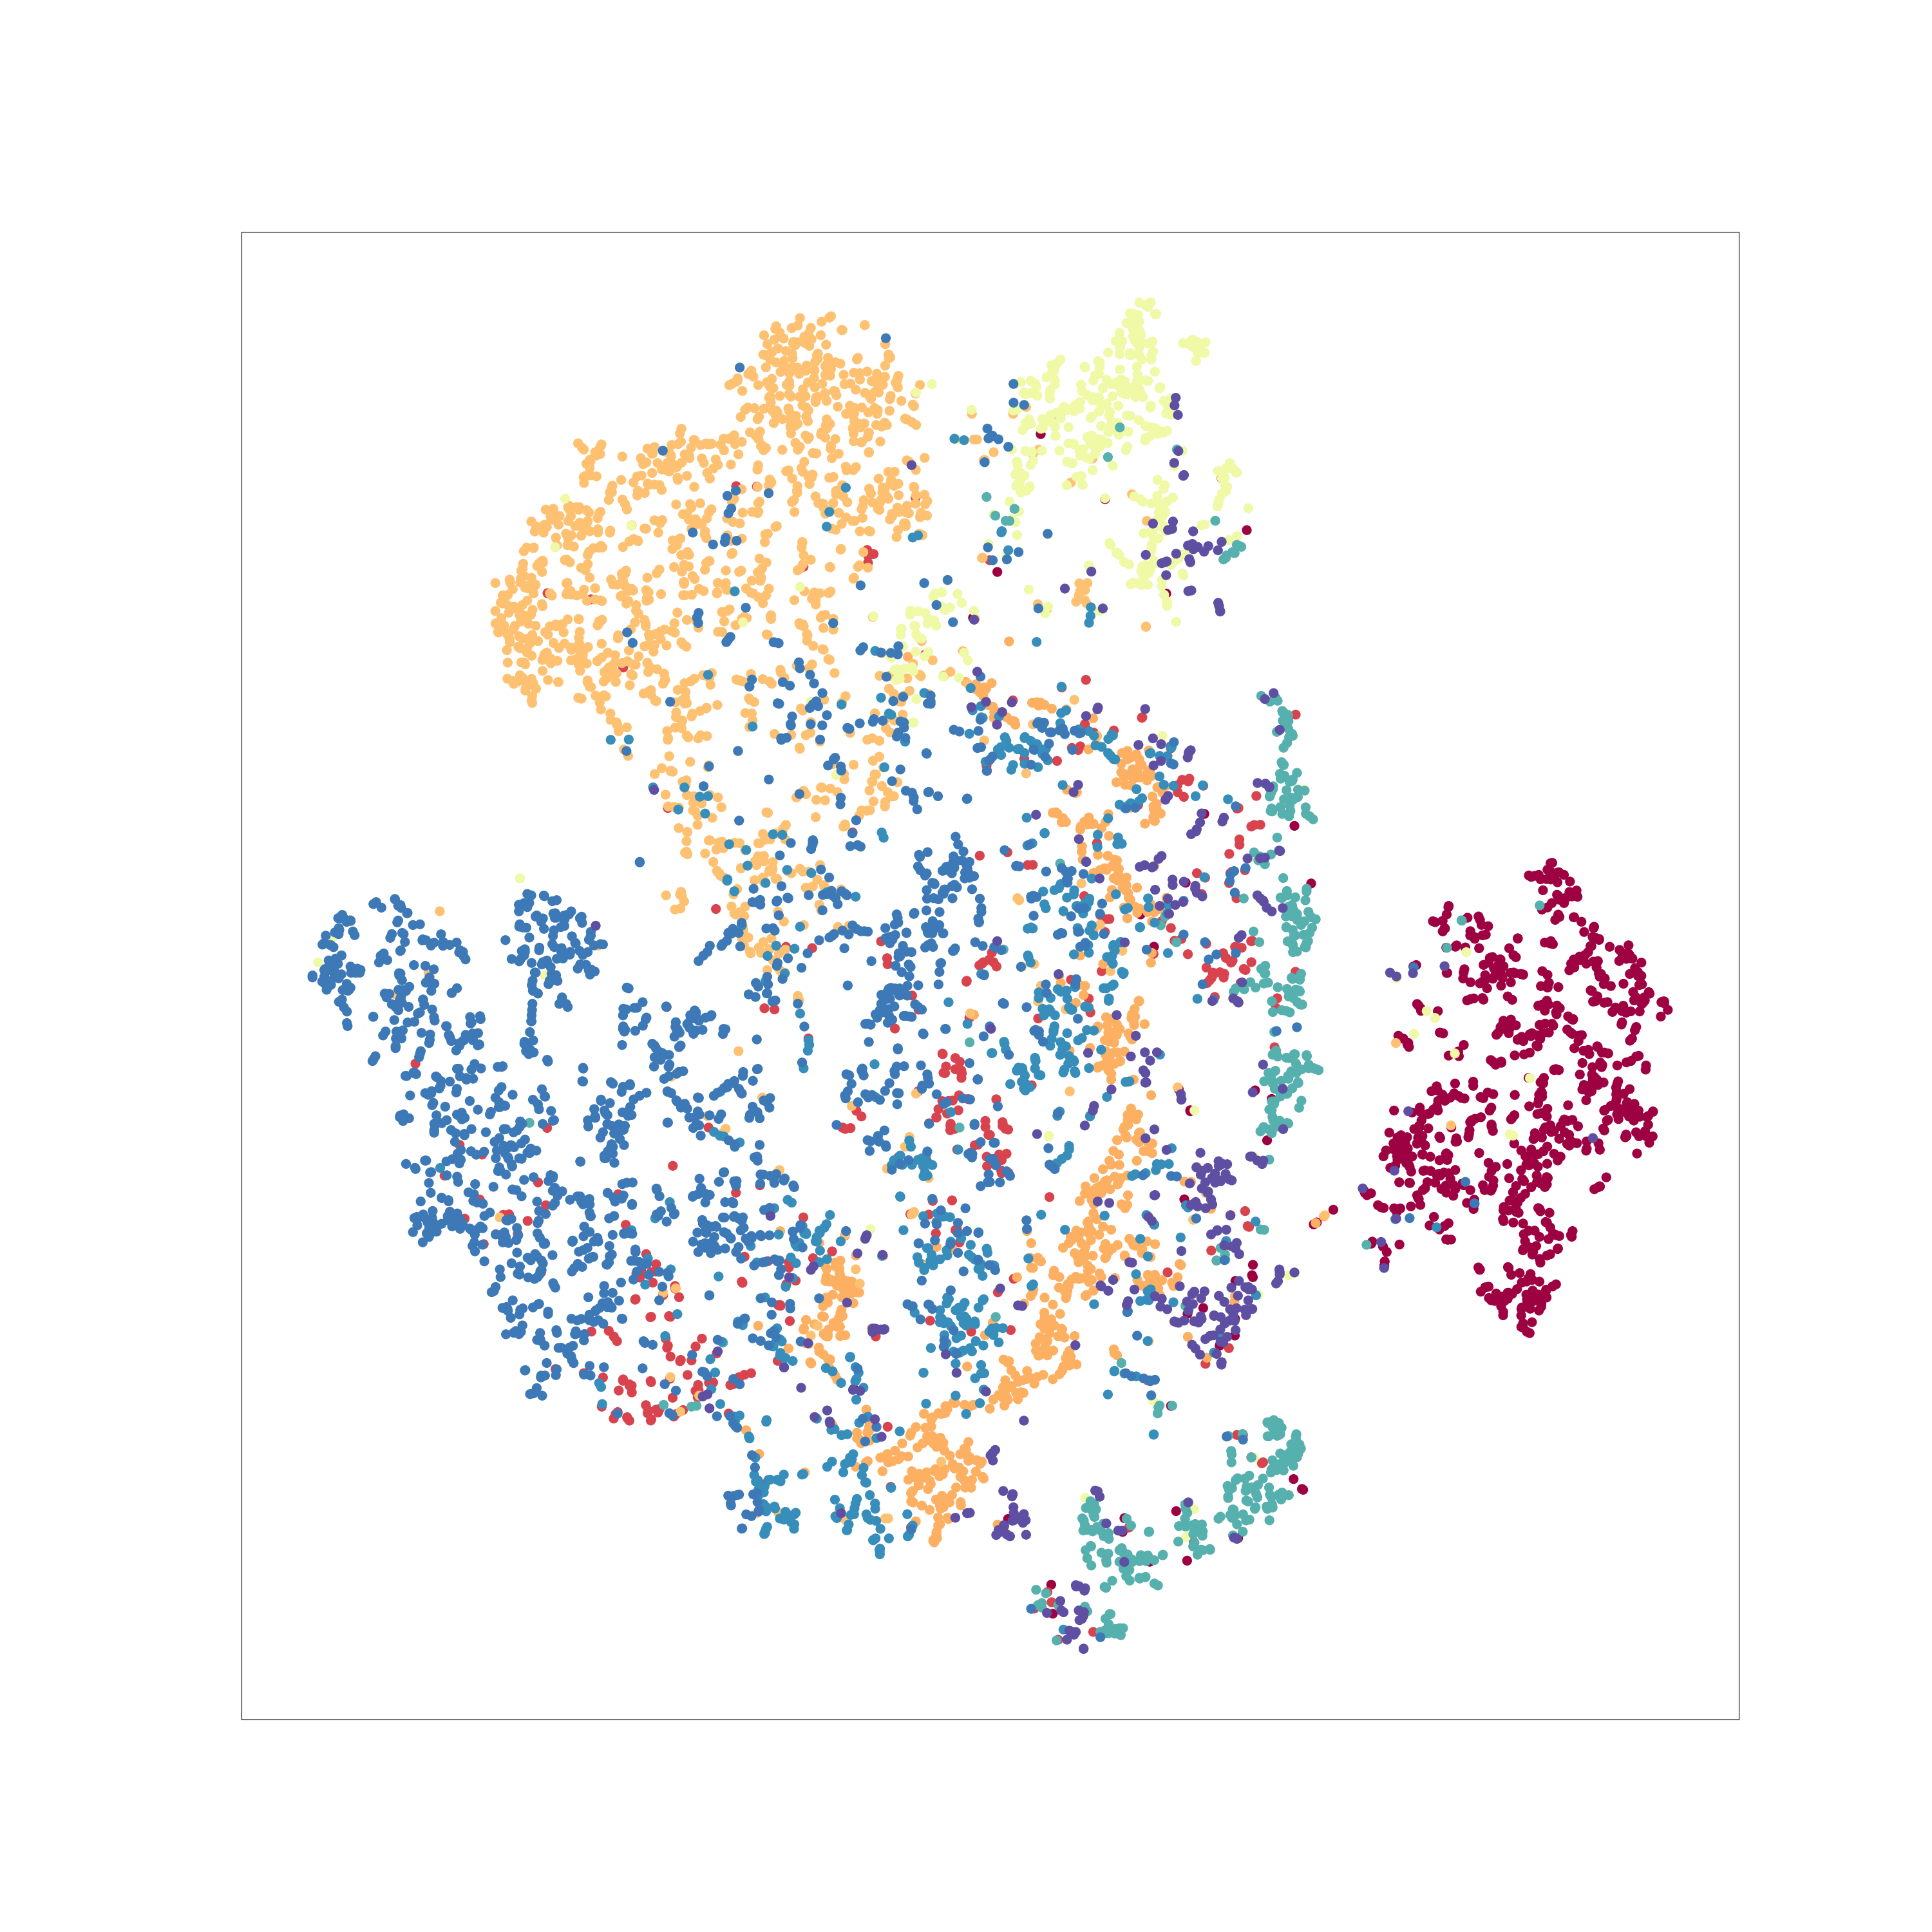
\includegraphics[width=\columnwidth]{figs/T-SNE-noclass.png}
    \caption{Without labels}\label{fig:T-SNE2}
  \end{subfigure}
  \hspace{0.05\linewidth}
  \begin{subfigure}[t]{0.2\linewidth} \centering
    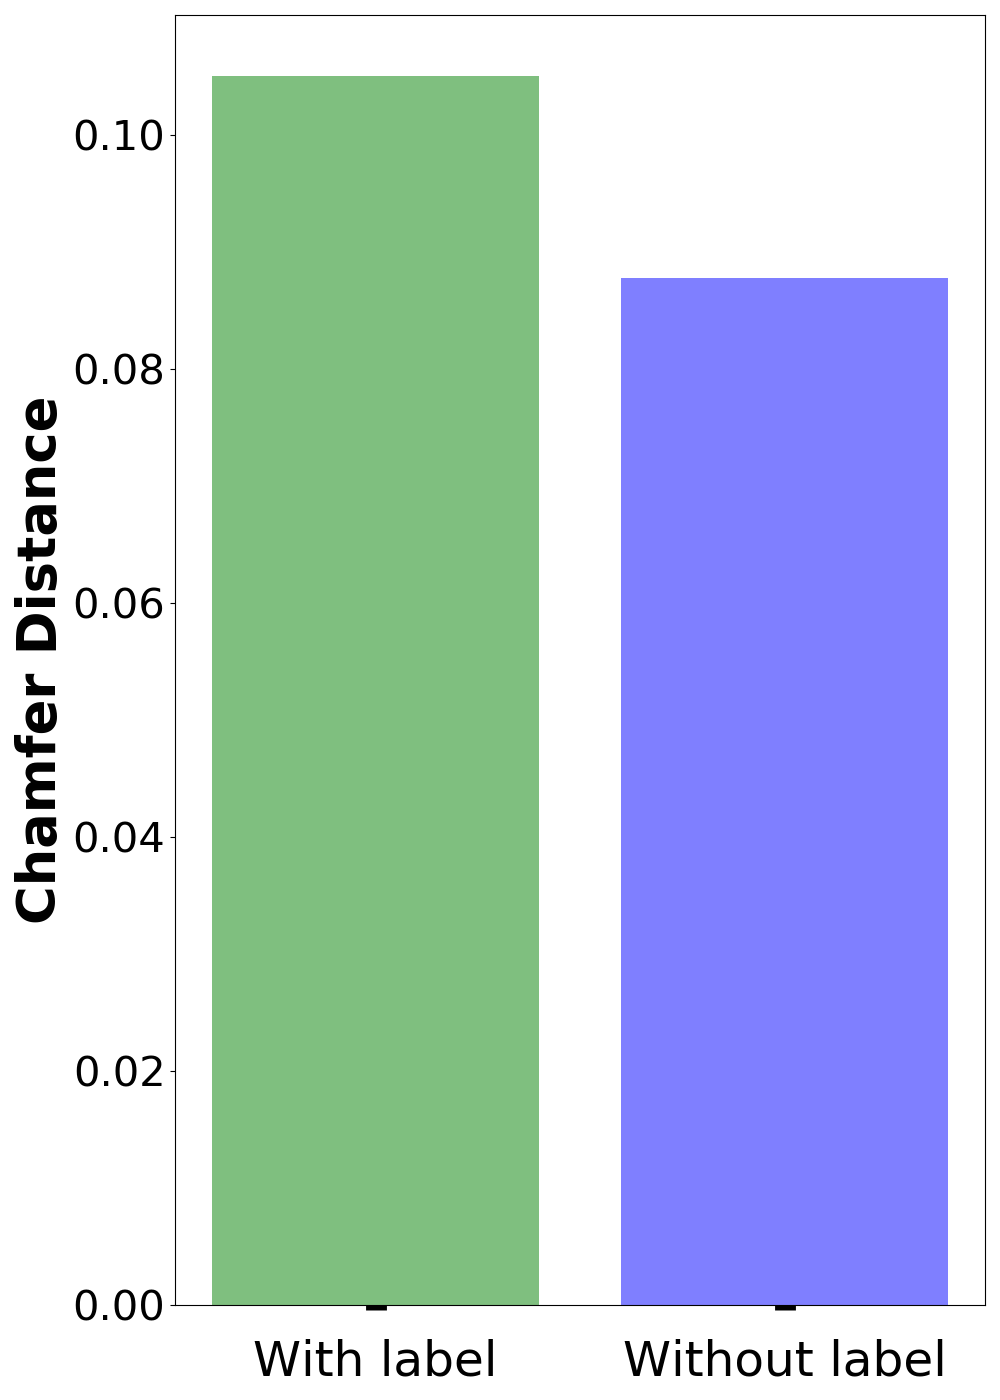
\includegraphics[width=\columnwidth]{figs/label-or-not.png}
    \caption{Chamfer loss}\label{fig:T-SNE3}
  \end{subfigure}
  \caption{\small T-SNE and Chamfer loss of the same network trained with or without label information. The network trained without label information does not show a clear tendency to form clusters while yielding smaller Chamfer loss.}\label{fig:T-SNE}
\end{figure}

\chapter{机制探究}
\section{理论分析}
\begin{figure}
    \centering
    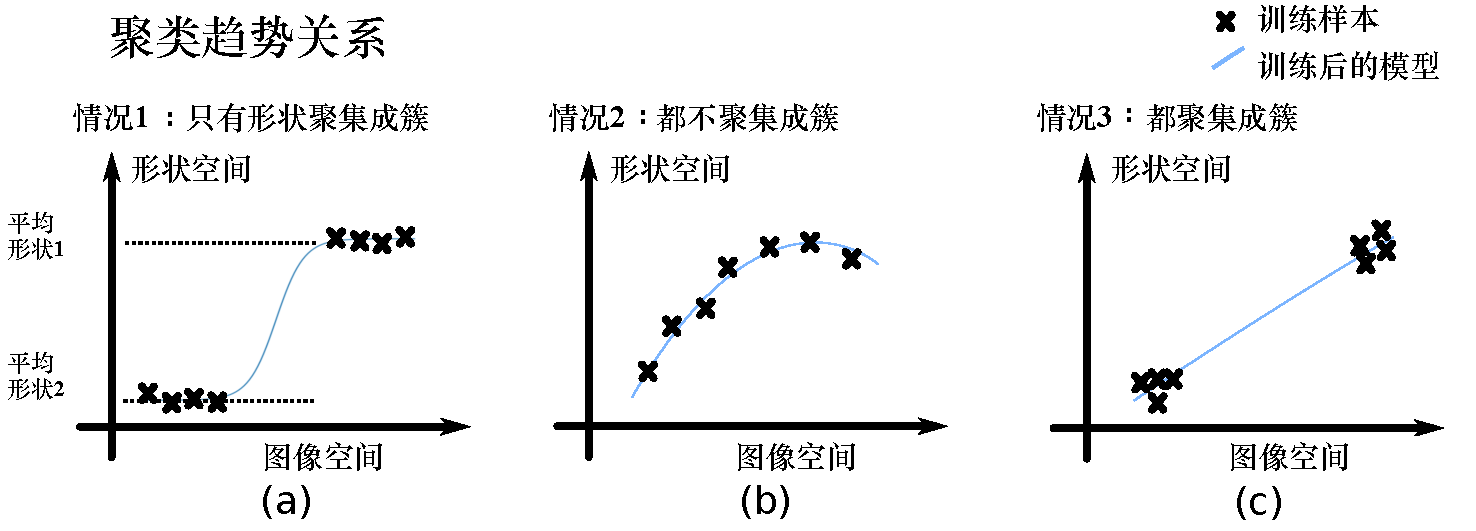
\includegraphics[width=.95\textwidth]{figs/drawing-1.pdf}
    \caption{\small When the training images are less clustered than the training shapes (as shown in subfigure (a)), the learned model shows the tendency of recognition.}
    \label{fig:clustering_tendency}
\end{figure}
\section{实验设计与数据集生成}
\begin{figure}
	\begin{tabular}{c@{}c@{}c@{}c@{}c@{}c@{}c@{}c@{}c@{}c@{}c@{}}
	    sphere & & & & & $\Longleftrightarrow$ & & & & & cube \\
		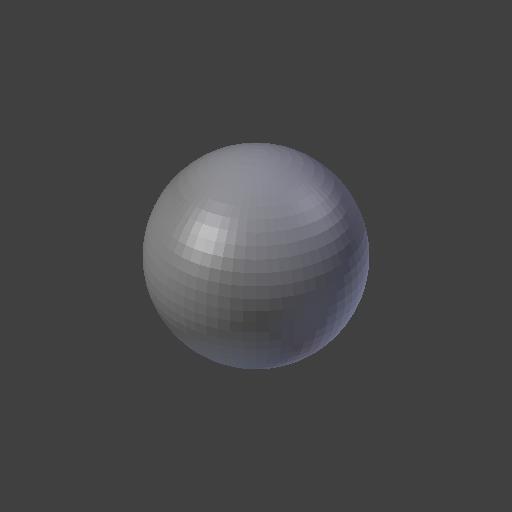
\includegraphics[width=.09\textwidth,keepaspectratio]{figs/Isometric0.png} &
		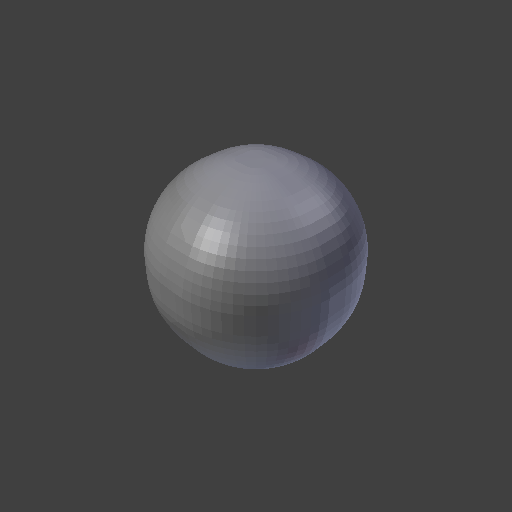
\includegraphics[width=.09\textwidth,keepaspectratio]{figs/Isometric1.png} &
		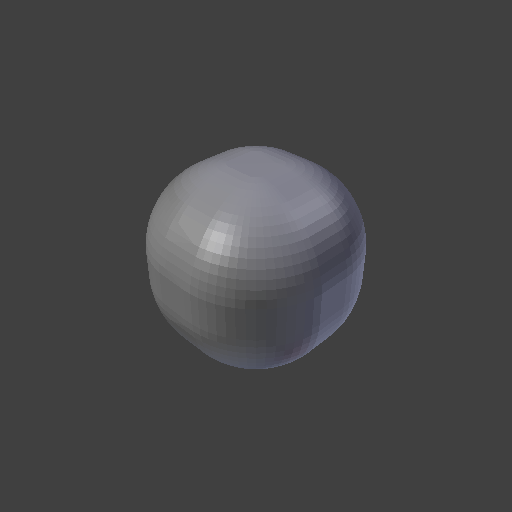
\includegraphics[width=.09\textwidth,keepaspectratio]{figs/Isometric2.png} &
		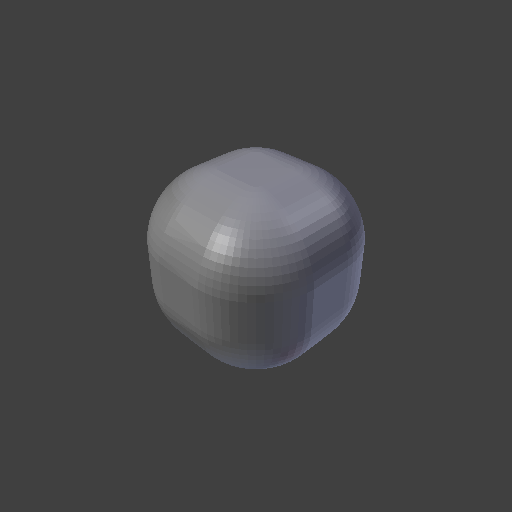
\includegraphics[width=.09\textwidth,keepaspectratio]{figs/Isometric3.png} &
		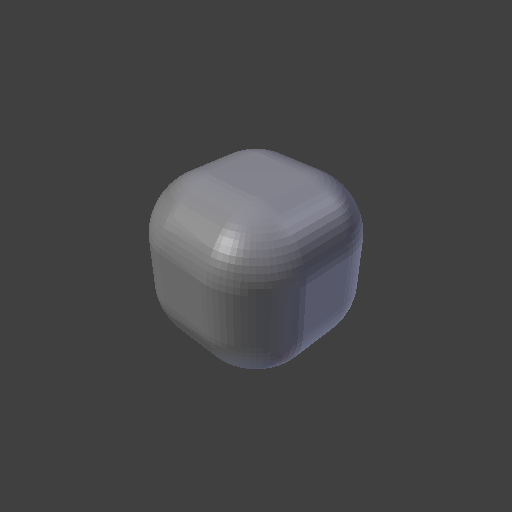
\includegraphics[width=.09\textwidth,keepaspectratio]{figs/Isometric4.png} &
		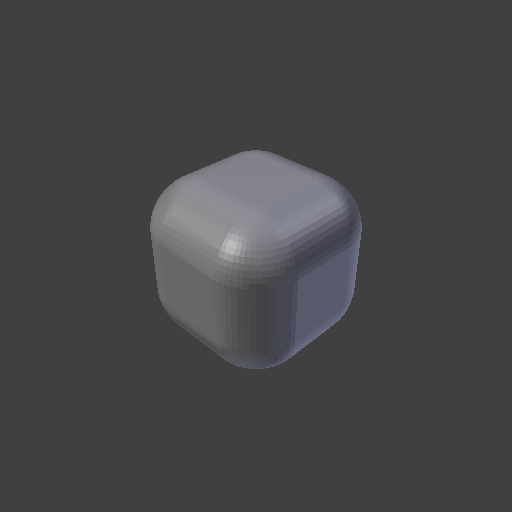
\includegraphics[width=.09\textwidth,keepaspectratio]{figs/Isometric5.png} &
		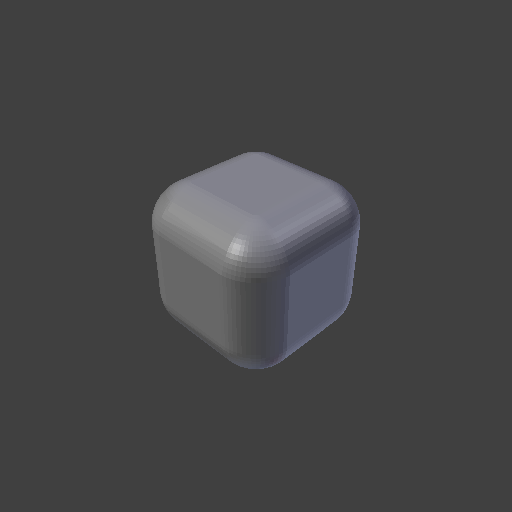
\includegraphics[width=.09\textwidth,keepaspectratio]{figs/Isometric6.png} &
		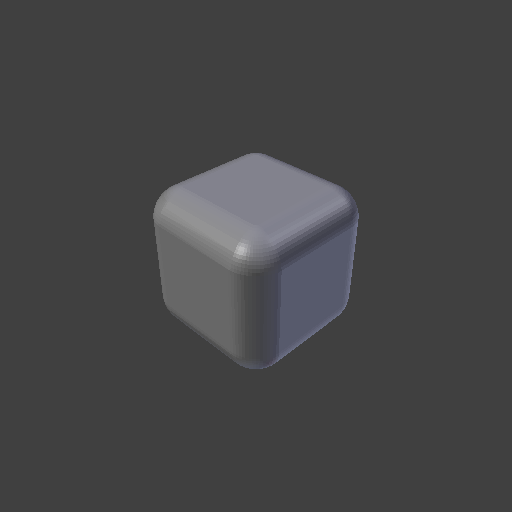
\includegraphics[width=.09\textwidth,keepaspectratio]{figs/Isometric7.png} &
		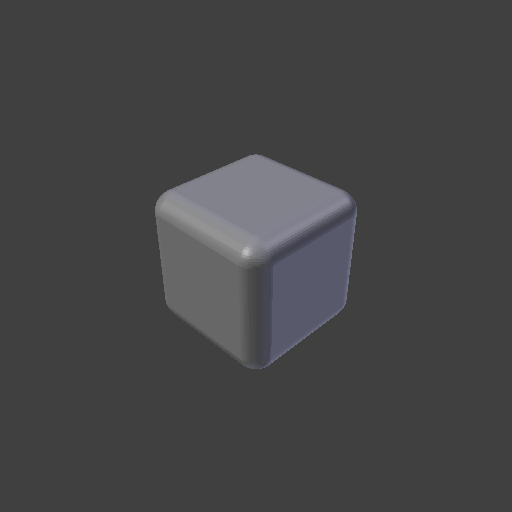
\includegraphics[width=.09\textwidth,keepaspectratio]{figs/Isometric8.png} &
		\includegraphics[width=.09\textwidth,keepaspectratio]{figs/Isometric9.png} &
		\includegraphics[width=.09\textwidth,keepaspectratio]{figs/Isometric10.png} \\    	
	\end{tabular}
	\caption{\small Base dataset \# 1: interpolation between a sphere and a cube.}
    \label{fig:cube-sphere} \vspace{-4mm}
\end{figure}

\begin{figure}
	\begin{subfigure}[t]{0.45\linewidth} \centering 
     \includegraphics[width=\columnwidth]{figs/five-clusters.png}
     \caption{\small Dataset 1.1.n (n = 1, 2, $\ldots $7). Different subsampled datasets are generated to have different clustering tendencies. }\label{fig:five-clusters}
   \end{subfigure}\hspace{0.05\textwidth}
   \begin{subfigure}[t]{0.45\linewidth} \centering
     \includegraphics[width=\columnwidth]{figs/two-clusters.png}
     \caption{Dataset 1.2.n (n = 1, 2, $\ldots $7). The dot markers represent image distribution, while the cross markers represent point cloud distribution.}\label{fig:two-clusters}
   \end{subfigure}
   \caption{\small Coverage of two subsampled data sets 1.1.n and 1.2.n.}
\end{figure}

\section{实验结果}
\begin{figure}[h!]
    \centering
    \includegraphics[width=.95\textwidth]{figs/silhouette-dataset-1.png}
    \caption{\small Training-vs-prediction silhouette scores. Only Case 1 (the points with large dataset indices shown in the bottom-left figure) shows high tendency towards recognition.}
    \label{fig:silhouette-dataset-1.png}
\end{figure}

\begin{figure}[ht!]
    \begin{centering}
        \begin{tabular}{cccc|cccc}
        \toprule
         &Images & GT & Recons. & Images & GT & Recons.& \\
        \toprule
        1.1.1 &\includegraphics[width=0.12\columnwidth,keepaspectratio]{figs/toyset_matrices/cluster_5by20_1_1.png} &
        \includegraphics[width=0.12\columnwidth,keepaspectratio]{figs/toyset_matrices/cluster_5by20_1_2.png} &
        \includegraphics[width=0.12\columnwidth,keepaspectratio]{figs/toyset_matrices/cluster_5by20_1_3.png} &  
        \includegraphics[width=0.12\columnwidth,keepaspectratio]{figs/toyset_matrices/cluster_2by10_1_1.png} &
        \includegraphics[width=0.12\columnwidth,keepaspectratio]{figs/toyset_matrices/cluster_2by10_1_2.png} &
        \includegraphics[width=0.12\columnwidth,keepaspectratio]{figs/toyset_matrices/cluster_2by10_1_3.png}& 1.2.1\\
        %& DI = 1 & & & DI = 1 & \\
        %\midrule
        1.1.2 &\includegraphics[width=0.12\columnwidth,keepaspectratio]{figs/toyset_matrices/cluster_5by20_2_1.png} &
        \includegraphics[width=0.12\columnwidth,keepaspectratio]{figs/toyset_matrices/cluster_5by20_2_2.png} &
        \includegraphics[width=0.12\columnwidth,keepaspectratio]{figs/toyset_matrices/cluster_5by20_2_3.png} &  
        \includegraphics[width=0.12\columnwidth,keepaspectratio]{figs/toyset_matrices/cluster_2by10_2_1.png} &
        \includegraphics[width=0.12\columnwidth,keepaspectratio]{figs/toyset_matrices/cluster_2by10_2_2.png} &
        \includegraphics[width=0.12\columnwidth,keepaspectratio]{figs/toyset_matrices/cluster_2by10_2_3.png}& 1.2.2\\
        %& DI = 2 & & & DI = 2 & \\
        %\midrule
        1.1.3 &\includegraphics[width=0.12\columnwidth,keepaspectratio]{figs/toyset_matrices/cluster_5by20_3_1.png} &
        \includegraphics[width=0.12\columnwidth,keepaspectratio]{figs/toyset_matrices/cluster_5by20_3_2.png} &
        \includegraphics[width=0.12\columnwidth,keepaspectratio]{figs/toyset_matrices/cluster_5by20_3_3.png} &  
        \includegraphics[width=0.12\columnwidth,keepaspectratio]{figs/toyset_matrices/cluster_2by10_3_1.png} &
        \includegraphics[width=0.12\columnwidth,keepaspectratio]{figs/toyset_matrices/cluster_2by10_3_2.png} &
        \includegraphics[width=0.12\columnwidth,keepaspectratio]{figs/toyset_matrices/cluster_2by10_3_3.png} & 1.2.3\\
        %& DI = 3 & & & DI = 3 & \\
        %\midrule
        1.1.4 &\includegraphics[width=0.12\columnwidth,keepaspectratio]{figs/toyset_matrices/cluster_5by20_4_1.png} &
        \includegraphics[width=0.12\columnwidth,keepaspectratio]{figs/toyset_matrices/cluster_5by20_4_2.png} &
        \includegraphics[width=0.12\columnwidth,keepaspectratio]{figs/toyset_matrices/cluster_5by20_4_3.png} &  
        \includegraphics[width=0.12\columnwidth,keepaspectratio]{figs/toyset_matrices/cluster_2by10_4_1.png} &
        \includegraphics[width=0.12\columnwidth,keepaspectratio]{figs/toyset_matrices/cluster_2by10_4_2.png} &
        \includegraphics[width=0.12\columnwidth,keepaspectratio]{figs/toyset_matrices/cluster_2by10_4_3.png} & 1.2.4\\
        %& DI = 4 & & & DI = 4 & \\
        %\midrule
        1.1.5 &\includegraphics[width=0.12\columnwidth,keepaspectratio]{figs/toyset_matrices/cluster_5by20_5_1.png} &
        \includegraphics[width=0.12\columnwidth,keepaspectratio]{figs/toyset_matrices/cluster_5by20_5_2.png} &
        \includegraphics[width=0.12\columnwidth,keepaspectratio]{figs/toyset_matrices/cluster_5by20_5_3.png} &  
        \includegraphics[width=0.12\columnwidth,keepaspectratio]{figs/toyset_matrices/cluster_2by10_5_1.png} &
        \includegraphics[width=0.12\columnwidth,keepaspectratio]{figs/toyset_matrices/cluster_2by10_5_2.png} &
        \includegraphics[width=0.12\columnwidth,keepaspectratio]{figs/toyset_matrices/cluster_2by10_5_3.png}& 1.2.5\\
        %& DI = 5 & & & DI = 5 & \\
        %\midrule
        1.1.6 &\includegraphics[width=0.12\columnwidth,keepaspectratio]{figs/toyset_matrices/cluster_5by20_6_1.png} &
        \includegraphics[width=0.12\columnwidth,keepaspectratio]{figs/toyset_matrices/cluster_5by20_6_2.png} &
        \includegraphics[width=0.12\columnwidth,keepaspectratio]{figs/toyset_matrices/cluster_5by20_6_3.png} &  
        \includegraphics[width=0.12\columnwidth,keepaspectratio]{figs/toyset_matrices/cluster_2by10_6_1.png} &
        \includegraphics[width=0.12\columnwidth,keepaspectratio]{figs/toyset_matrices/cluster_2by10_6_2.png} &
        \includegraphics[width=0.12\columnwidth,keepaspectratio]{figs/toyset_matrices/cluster_2by10_6_3.png}& 1.2.6\\
        %& DI = 6 & & & DI = 6 & \\
        %\midrule
        1.1.7 &\includegraphics[width=0.12\columnwidth,keepaspectratio]{figs/toyset_matrices/cluster_5by20_7_1.png} &
        \includegraphics[width=0.12\columnwidth,keepaspectratio]{figs/toyset_matrices/cluster_5by20_7_2.png} &
        \includegraphics[width=0.12\columnwidth,keepaspectratio]{figs/toyset_matrices/cluster_5by20_7_3.png} &  
        \includegraphics[width=0.12\columnwidth,keepaspectratio]{figs/toyset_matrices/cluster_2by10_7_1.png} &
        \includegraphics[width=0.12\columnwidth,keepaspectratio]{figs/toyset_matrices/cluster_2by10_7_2.png} &
        \includegraphics[width=0.12\columnwidth,keepaspectratio]{figs/toyset_matrices/cluster_2by10_7_3.png} & 1.2.7\\
        %& DI = 7 & & & DI = 7 & \\
        \bottomrule  
        \end{tabular}  \vspace{-2mm}
        \caption{\small Distance matrices. Blue represents small distance and red represents large distance. {\bf (Left)} predicted shapes of subsampled dataset 1.1 are not clustered. {\bf (Right)} predicted shapes of subsampled dataset 1.2 are clustered if the training images are not clustered (i.e., if the dataset belongs to Case 1). Top to bottom: dataset index from 1 to 7.}
        \label{fig:cluster_visualization}
    \end{centering}
    \end{figure}


\end{Main} % 结束正文

% 参考文献

\bibliography{seuthesis}

%附录
\begin{Appendix}{}
    \chapter{{\LaTeX}实验}
    技术实验结果在这里写
    \chapter{MATLAB实验}
    技术实验结果在这里写
\end{Appendix}

\begin{Acknowledgement}{}
    这次的毕业论文设计总结是在我的指导老师xxx老师亲切关怀和悉心指导下完成的。从毕业设计选题到设计完成,x老师给予了我耐心指导与细心关怀,有了莫老师耐心指导与细心关怀我才不会在设计的过程中迷失方向,失去前进动力。x老师有严肃的科学态度,严谨的治学精神和精益求精的工作作风,这些都是我所需要学习的,感谢x老师给予了我这样一个学习机会,谢谢!

    感谢与我并肩作战的舍友与同学们,感谢关心我支持我的朋友们,感谢学校领导、老师们,感谢你们给予我的帮助与关怀;感谢肇庆学院,特别感谢计算机科学与软件学院四年来为我提供的良好学习环境,谢谢!
\end{Acknowledgement}

\newpage
\printindex % 索引

%\begin{thebibliography}{99}


%\bibliographystyle{ieee}
%\bibliography{seuthesis}


\end{document}
